\documentclass[compress]{beamer}
\usepackage{ifthen,verbatim}

\title{Track-based Muon Alignment: \\ Updated Procedures, Tools, \\ and Systematics Studies}
\author{Jim Pivarski, Alexei Safonov, Karoly Banicz, Vadim Khotilovich}
\institute{Texas A\&M University}
\date{18 September, 2007}

\newcommand{\isnote}{}
\xdefinecolor{lightyellow}{rgb}{1.,1.,0.25}
\xdefinecolor{darkblue}{rgb}{0.1,0.1,0.7}

%% Uncomment this to get annotations
%% \def\notes{\addtocounter{page}{-1}
%%            \renewcommand{\isnote}{*}
%% 	   \beamertemplateshadingbackground{lightyellow}{white}
%%            \begin{frame}
%%            \frametitle{Notes for the previous page (page \insertpagenumber)}
%%            \itemize}
%% \def\endnotes{\enditemize
%% 	      \end{frame}
%%               \beamertemplateshadingbackground{white}{white}
%%               \renewcommand{\isnote}{}}

%% Uncomment this to not get annotations
\def\notes{\comment}
\def\endnotes{\endcomment}

\setbeamertemplate{navigation symbols}{}
\setbeamertemplate{headline}{\includegraphics[height=1 cm]{../cmslogo} \hspace{0.1 cm} \includegraphics[height=1 cm]{../tamulogo} \hfill
\begin{minipage}{5.5 cm}
\vspace{-0.75 cm} \small
\begin{center}
\ifthenelse{\equal{\insertpagenumber}{1}}{}{\textcolor{blue}{\insertsection}}
\end{center}
\end{minipage} \hfill
\begin{minipage}{4.5 cm}
\vspace{-0.75 cm} \small
\begin{flushright}
\ifthenelse{\equal{\insertpagenumber}{1}}{}{Jim Pivarski \hspace{0.5 cm} \insertpagenumber\isnote/\pageref{numpages}}
\end{flushright}
\end{minipage}\mbox{\hspace{0.2 cm}}}

\begin{document}
\frame{\titlepage}

\begin{notes}
\item This is the annotated version of my talk.
\item If you want the version that I am presenting, download the one
labeled ``slides'' on Indico (or just ignore these yellow pages).
\item The annotated version is provided for extra detail and a written
record of comments that I intend to make orally.
\item Yellow notes refer to the content on the {\it previous} page.
\item All other slides are identical for the two versions.
\end{notes}

\begin{frame}
\frametitle{Overview}
\vspace{-0.75 cm}
\renewcommand{\arraystretch}{1.6}
\begin{tabular}{p{0.7\linewidth} p{0.25\linewidth}}
& Status \\ \hline

Infrastructure for online alignment

\vspace{0.1 cm}
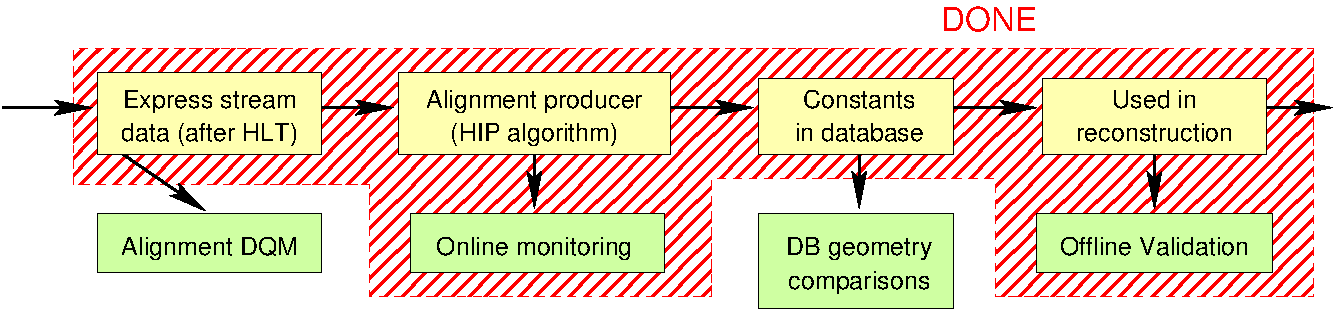
\includegraphics[width=\linewidth]{online_alignment.pdf} & Central path is done;
work on DB monitor has resumed \\

Systematics studies & Some completed \\

Background studies; finalize cuts & CSA07 exercise \\\hline

Beam-halo alignment (Karoly Banicz) & \mbox{Checking} \mbox{feasibility} \\ \hline

Cosmic ray and MTCC alignment

(Alexey~Kamenev) & Near future \\
\end{tabular}
\end{frame}

\begin{frame}
\frametitle{What we're focusing on and why}
Present
\begin{itemize}\setlength{\itemsep}{0.2 cm}
\item \textcolor{darkblue}{Monitoring:} to catch and fix mistakes quickly
\item \textcolor{darkblue}{Systematics studies:} quantify complicating effects and make sure
they're not show-stoppers
\item \textcolor{darkblue}{Beam-halo alignment:} potential opportunity to align all CSC
layers with tracks before first collisions
\end{itemize}

\uncover<2>{Near future
\begin{itemize}\setlength{\itemsep}{0.2 cm}
\item \textcolor{darkblue}{Background studies:} loosen event selection from $Z\to\mu\mu$ to
an inclusive $p_T$ cut.  Requires a realistic event sample with all
backgrounds, which we can get from CSA07.

\item \textcolor{darkblue}{MTCC:} real data, includes $\vec{B}(t)$ and
an opportunity to connect track-based alignment with photogrammetry
and laser system.  Data must be re-processed in a 1\_5\_X+ release.
\end{itemize}}
\end{frame}

\section*{Monitoring alignment changes}

\begin{frame}
\begin{center}
\Huge \textcolor{blue}{Monitoring alignment changes \\ in the database}
\end{center}
\end{frame}

\begin{frame}
\frametitle{Examples from DB geometry comparison tool (1 of 2)}
\begin{itemize}
\item Comparison of real alignment output (blue line) with a misalignment scenario (filled green)
\end{itemize}
\begin{center}
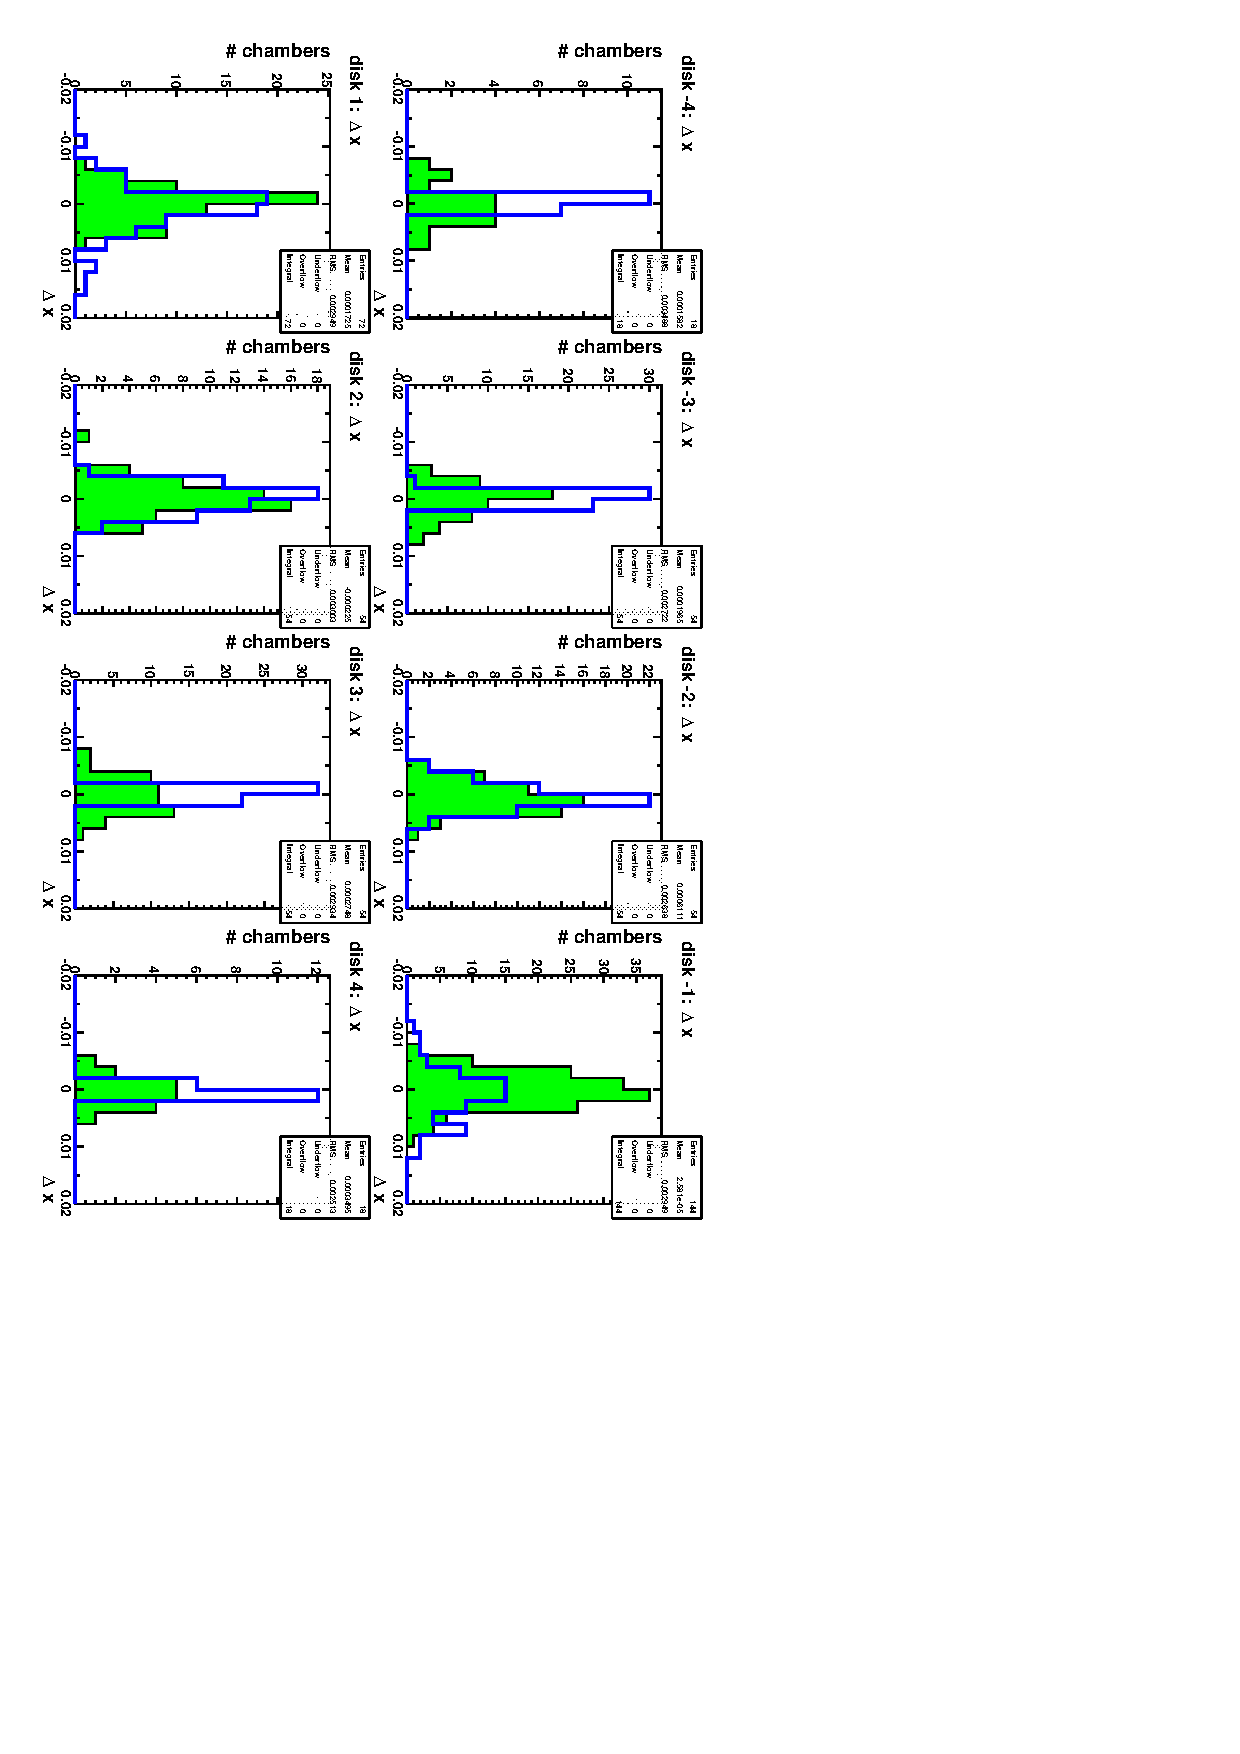
\includegraphics[height=0.9\linewidth, angle=90]{c_endcap_dxloc_overlay.pdf}

Aligned $-$ ideal local $x$ in endcap
\end{center}
\end{frame}

\begin{frame}
\frametitle{Examples from DB geometry comparison tool (2 of 2)}
\begin{itemize}
\item Time series of increasing misalignment

\item (Response to misalignment of tracker: we'll see more later)
\end{itemize}

\vfill
\begin{center}
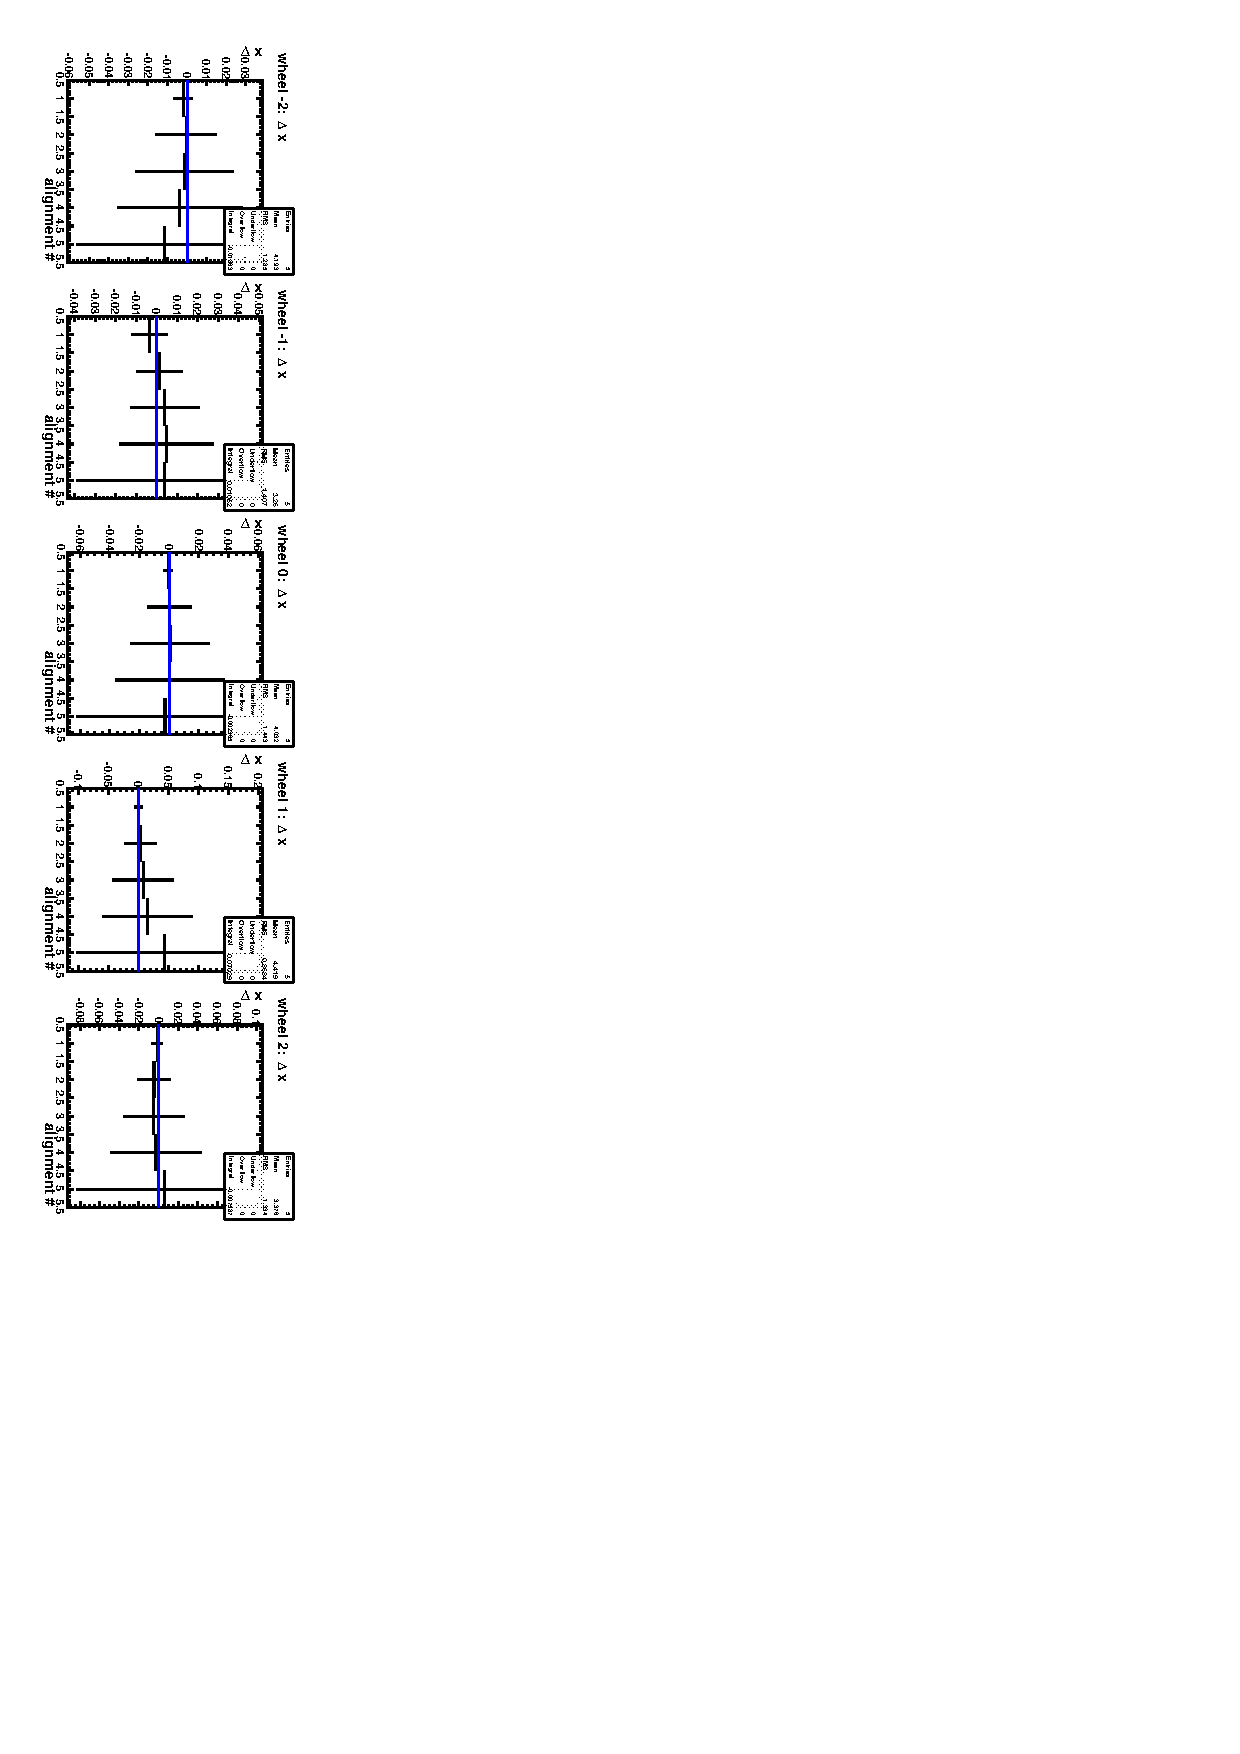
\includegraphics[height=\linewidth, angle=90]{c_barrel_dxloc.pdf}

\vspace{0.25 cm}
RMS of aligned $-$ ideal global $z$ in barrel
\end{center}

\vfill
\textcolor{darkblue}{New student: Vadim Khotilovich}
\end{frame}

\section*{Optimized procedure}

\begin{frame}
\begin{center}
\Huge \textcolor{blue}{Optimized alignment procedure}
\end{center}
\end{frame}

\begin{frame}
\frametitle{Hierarchical 2--3 step process}

\begin{enumerate}\setlength{\itemsep}{0.3 cm}
\item Determine wheel/disk positions to 0.7~mm accuracy \\ with
a few hundred muons
\item Determine chamber positions to 100~$\mu$m with 10~pb$^{-1}$
\item Determine CSC layer positions, if necessary
\end{enumerate}
\begin{center}
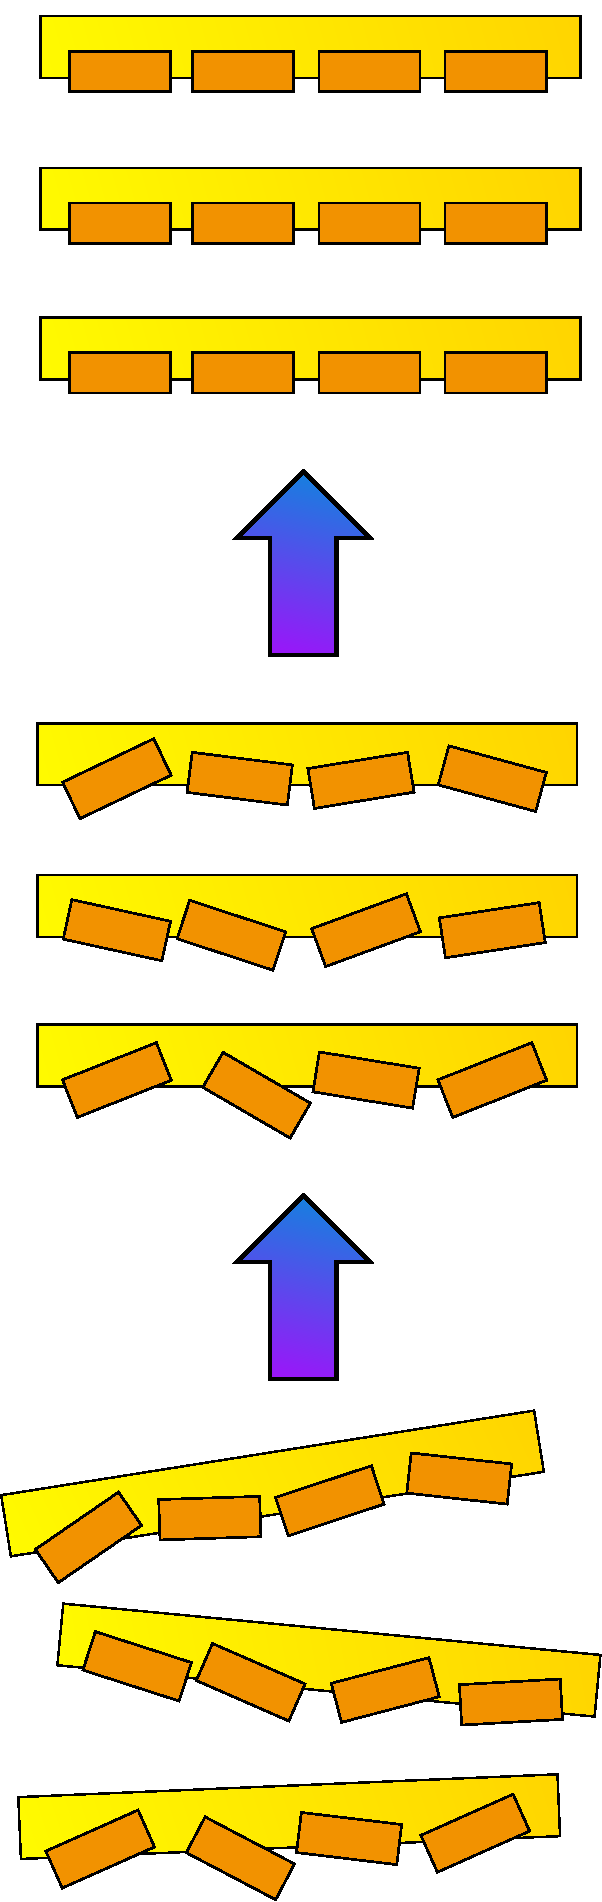
\includegraphics[height=\linewidth, angle=-90]{heirarchial_procedure.pdf}
\end{center}
\end{frame}

\begin{frame}
\frametitle{Degrees of freedom: barrel wheels}
\begin{columns}
\column{0.5\linewidth}
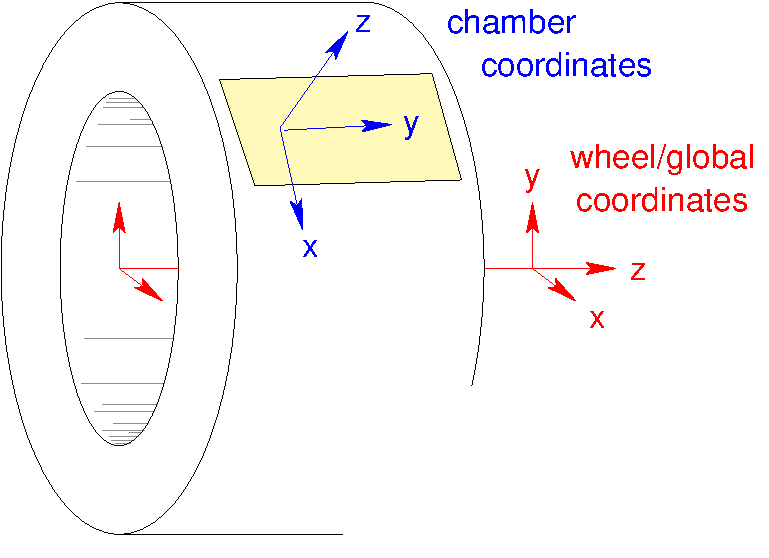
\includegraphics[height=4 cm]{wheel_parameters.pdf}
\column{0.5\linewidth}
\begin{center}
All 6 float in alignment

\vspace{1 cm}
\mbox{ }
\end{center}
\end{columns}

\vspace{-1.2 cm}
\mbox{ } \hfill \renewcommand{\arraystretch}{1.2} \begin{tabular}{c c}
Wheel coordinate & Chamber residual \\\hline\hline
$\phi_z$ & $x$ residual \\
$x$, $y$ & linear combination of $x$ and $y$ \\\hline
$z$ & $y$ residual \\
$\phi_y$ & left$-$right $y$ differences \\
$\phi_y$ & top$-$bottom $y$ differences \\
\end{tabular}
\end{frame}

\begin{frame}
\frametitle{Degrees of freedom: endcap disks}
\begin{columns}
\column{0.5\linewidth}
\mbox{ } \hspace{0.5 cm} 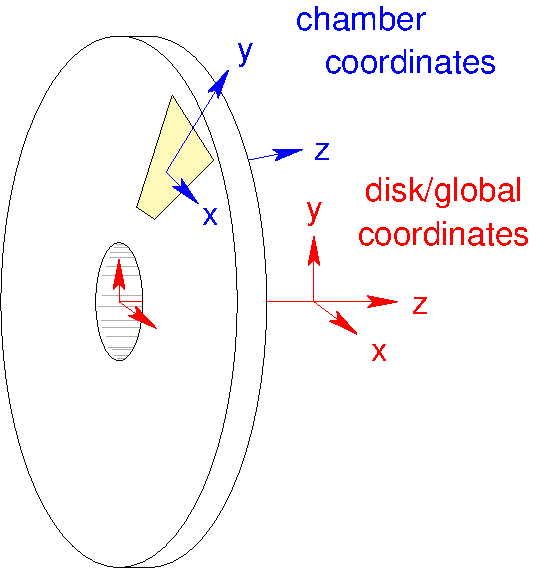
\includegraphics[height=4 cm]{disk_parameters.pdf}
\column{0.5\linewidth}
\begin{center}
Only $x$, $y$, and $\phi_z$ float

\vspace{1 cm}
\mbox{ }
\end{center}
\end{columns}

\vspace{-0.7 cm}
\mbox{ } \hfill \renewcommand{\arraystretch}{1.2} \begin{tabular}{c c}
Disk coordinate & Chamber residual \\\hline\hline
$\phi_z$ & $x$ residual \\
$x$, $y$ & linear combination of $x$ and $y$ \\\hline
$z$ & $y$ residual differences\ldots \\
& (weakly constrained)
\end{tabular}
\end{frame}

\begin{frame}
\frametitle{Wheel/disk alignment results $\times$ 10 trials}
\hfill \begin{tabular}{c c}
$x$, $y$ positions & 0.71~mm \\
$z$ positions (barrel only) & 0.89~mm \\
$\phi_x$, $\phi_y$ angles (barrel only) & 0.20~mrad \\
$\phi_z$ angle & 0.11~mrad
\end{tabular}

\vfill
\begin{columns}
\column{0.6\linewidth}
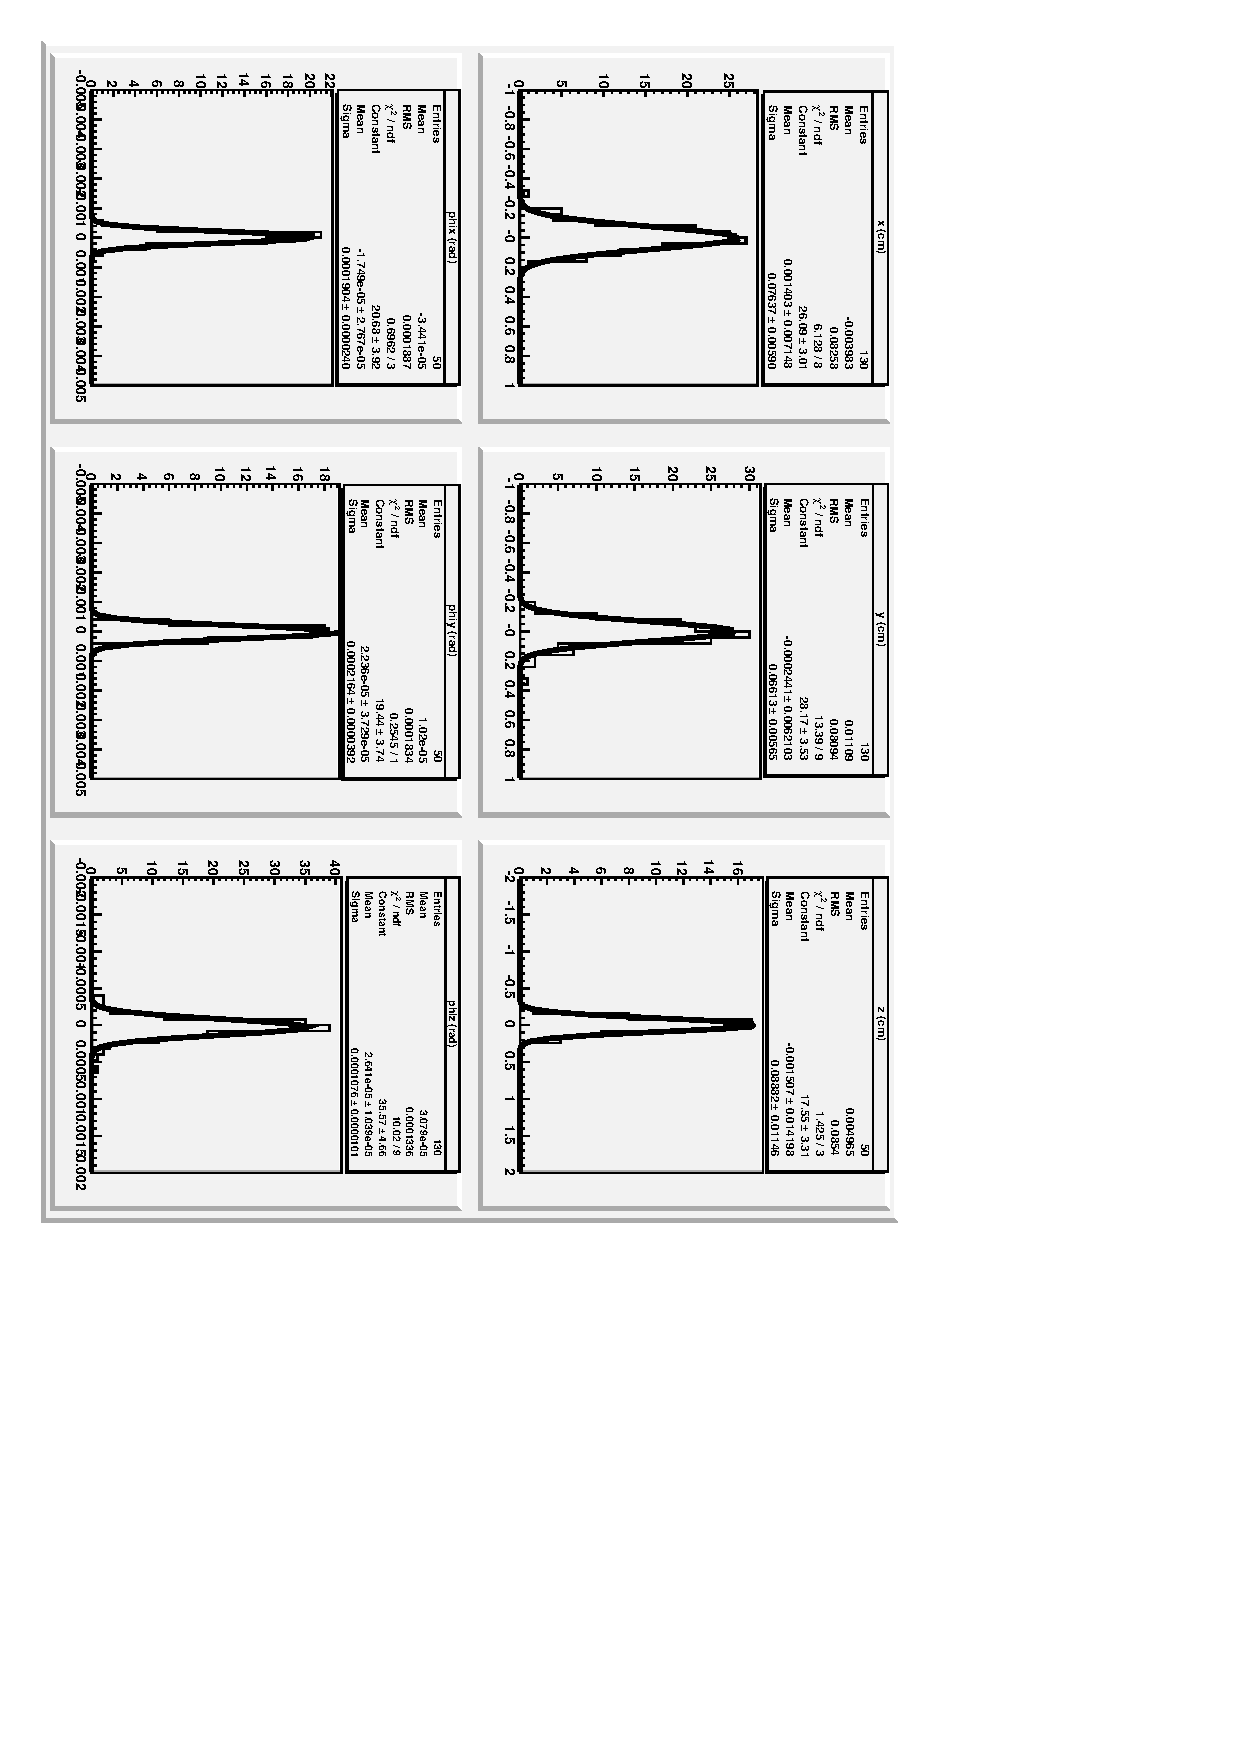
\includegraphics[height=0.9\linewidth, angle=90]{optimal_disk_alignment.pdf}

\column{0.4\linewidth}
6 d.o.f.\ float in barrel

only $x$, $y$, $\phi_z$ in endcap
\end{columns}

\vfill
Independent of the number of muons (``brick wall'' is $\sim$20 tracks)
\end{frame}

\begin{frame}
\frametitle{Chamber-by-chamber alignment}
\vspace{-1 cm}
\begin{center}
\begin{tabular}{p{0.31\linewidth} p{0.31\linewidth} p{0.31\linewidth}}
  \begin{minipage}{\linewidth}
    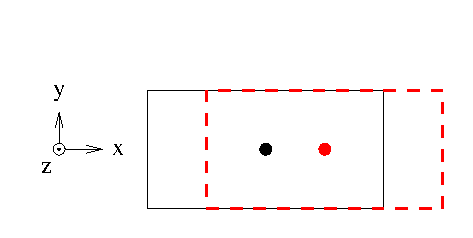
\includegraphics[width=\linewidth]{dof_x.pdf}
  \end{minipage} &
  \begin{minipage}{\linewidth}
    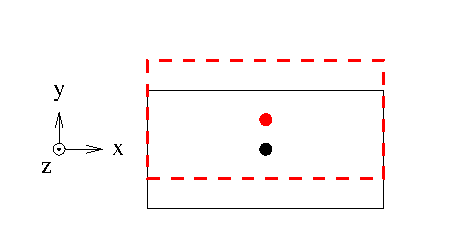
\includegraphics[width=\linewidth]{dof_y.pdf}
  \end{minipage} &
  \begin{minipage}{\linewidth}
    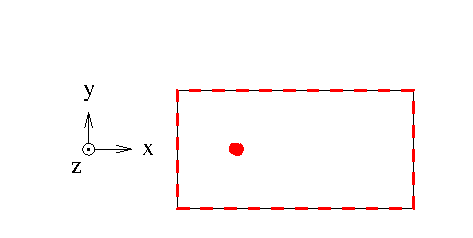
\includegraphics[width=\linewidth]{dof_z.pdf}
  \end{minipage} \\
  \begin{minipage}{\linewidth}
    \begin{center}
      $x$: offset in $r_x$
    \end{center}
  \end{minipage} &
  \begin{minipage}{\linewidth}
    \begin{center}
      $y$: offset in $r_y$
    \end{center}
  \end{minipage} &
  \begin{minipage}{\linewidth}
    \begin{center}
      $z$: via angled tracks
    \end{center}
  \end{minipage} \\
  \begin{minipage}{\linewidth}
    \tiny
    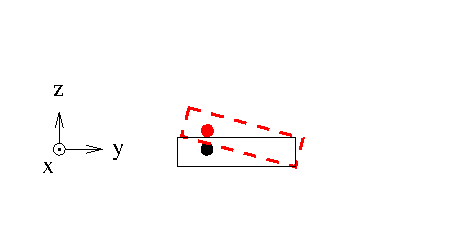
\includegraphics[width=\linewidth]{dof_phix.pdf}
  \end{minipage} &
  \begin{minipage}{\linewidth}
    \tiny
    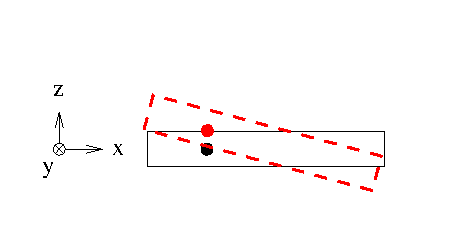
\includegraphics[width=\linewidth]{dof_phiy.pdf}
  \end{minipage} &
  \begin{minipage}{\linewidth}
    \tiny
    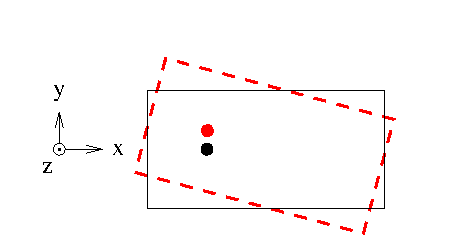
\includegraphics[width=\linewidth]{dof_phiz.pdf}
  \end{minipage} \\
  \begin{minipage}{\linewidth}
    \begin{center}
      $\phi_x$: $r_y$ linear in $y$
    \end{center}
  \end{minipage} &
  \begin{minipage}{\linewidth}
    \begin{center}
      $\phi_y$: $r_x$ linear in $x$
    \end{center}
  \end{minipage} &
  \begin{minipage}{\linewidth}
    \begin{center}
      $\phi_z$: $r_x$ linear in $y$
    \end{center}
  \end{minipage} \\
  \begin{minipage}{\linewidth}
    \scriptsize
    \begin{center}
      (slope $\propto$ $1 - \cos\phi_x$)
    \end{center}
  \end{minipage} &
  \begin{minipage}{\linewidth}
    \scriptsize
    \begin{center}
      (slope $\propto$ $1 - \cos\phi_y$)
    \end{center}
  \end{minipage} &
  \begin{minipage}{\linewidth}
    \scriptsize
    \begin{center}
      (slope $\propto$ $\sin\phi_z$)
    \end{center}
  \end{minipage}
\end{tabular}
\end{center}

\begin{itemize}
\item Barrel stations 1--3: all 6 parameters float
\item Barrel station 4 has no $y$ measurement: $x$, $\phi_y$, and $\phi_z$ only
\item ME 1/1: could not find an optimal set--- possible software bug
\item Other endcap: all but $\phi_x$
\end{itemize}
\end{frame}

\begin{frame}
\frametitle{Barrel chamber results \hfill {\small (MB4 not shown)}}
\vspace{-0.25 cm}
\begin{center}
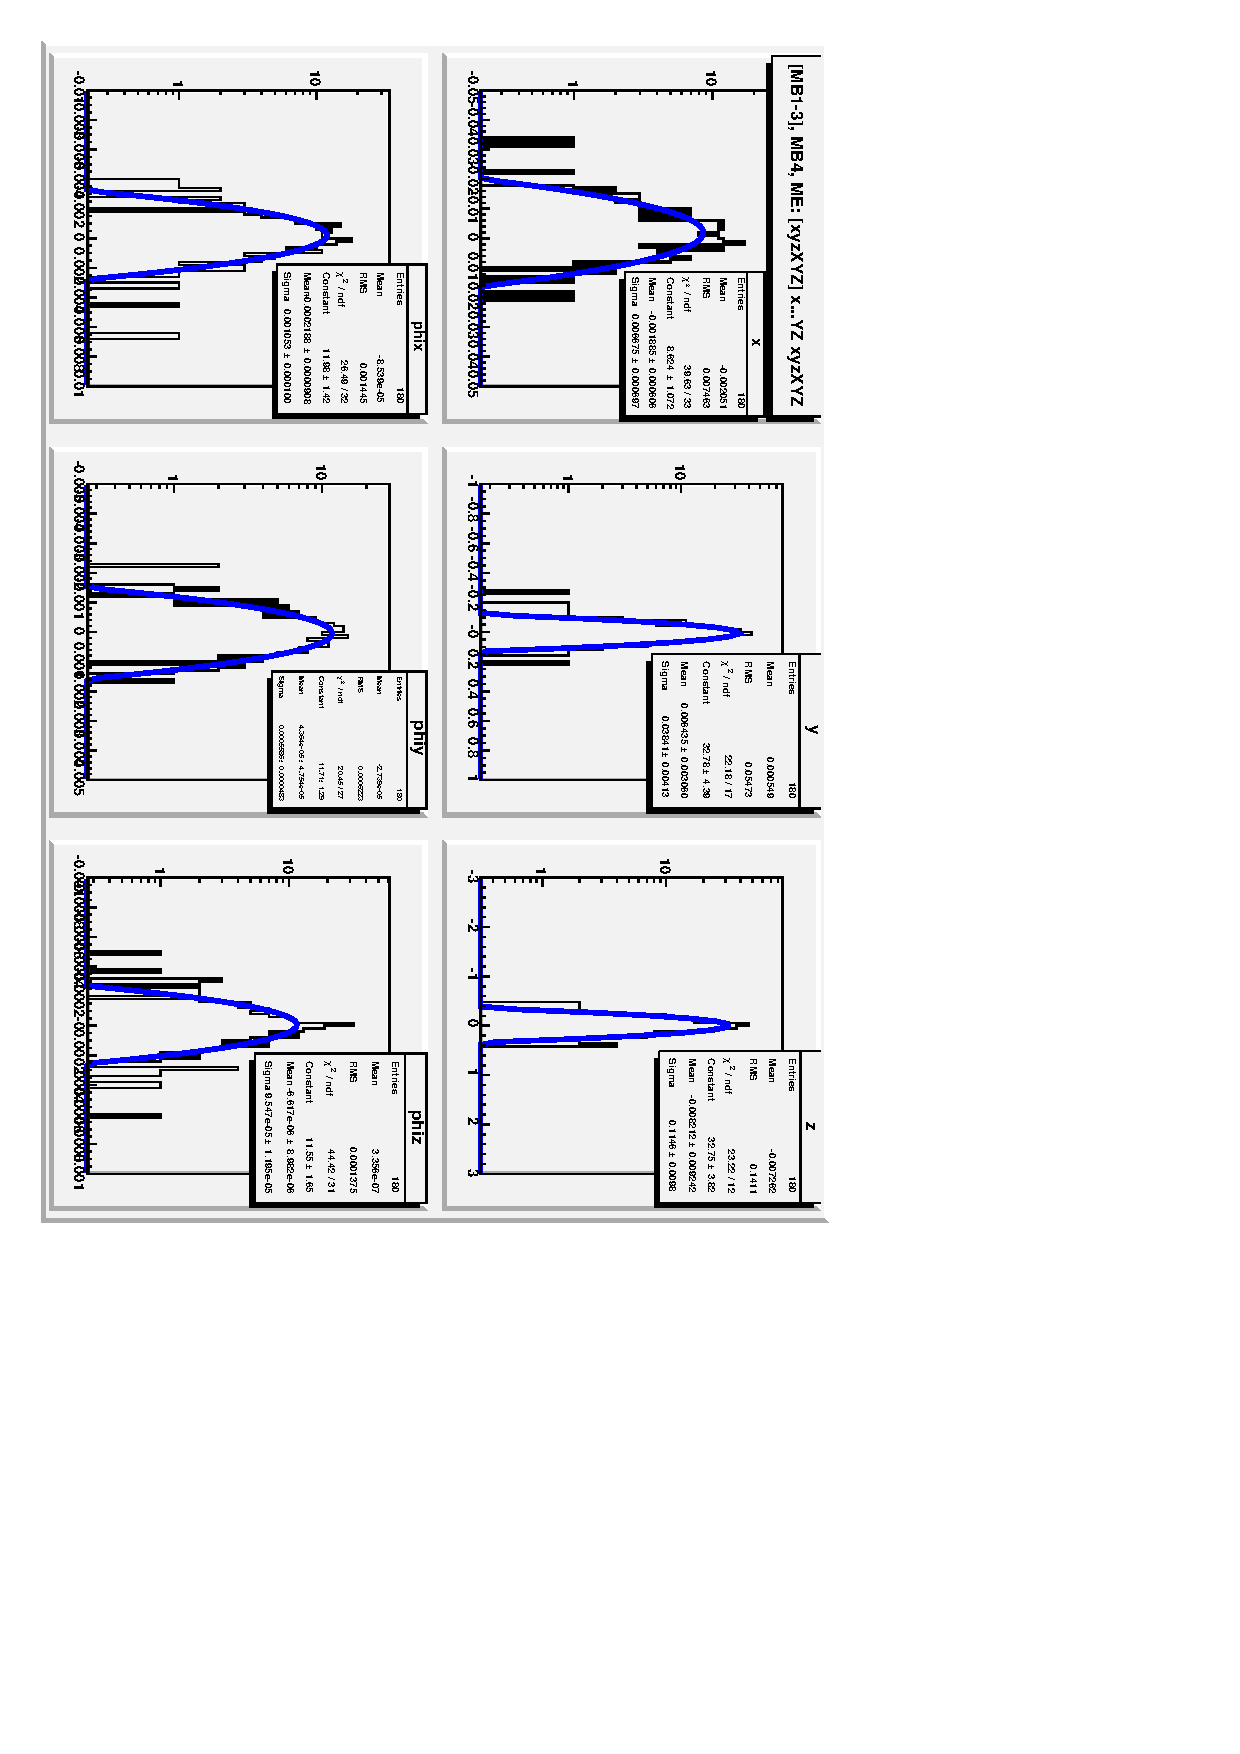
\includegraphics[height=0.7\linewidth, angle=90]{optimal_barrel_alignment.pdf}
\end{center}

\vspace{-0.75 cm}
\begin{columns}
\column{0.5\linewidth}
\begin{center}
MB 1--3
\begin{tabular}{c c | c c}
\hline\hline
$x$ & 67 $\mu$m & 1.05 mrad & $\phi_x$ \\
$y$ & 384 $\mu$m & 0.56 mrad & $\phi_y$ \\
$z$ & 1.15 mm & 0.095 mrad & $\phi_z$ \\
\hline\hline
\end{tabular}
\end{center}

\column{0.5\linewidth}
\begin{center}
MB 4
\begin{tabular}{c c | c c}
\hline\hline
$x$ & 28 $\mu$m &  \\
    &           & 0.57 mrad & $\phi_y$ \\
    &           & 0.004 mrad & $\phi_z$ \\
\hline\hline
\end{tabular}
\end{center}
\end{columns}
\end{frame}

\begin{frame}
\frametitle{Endcap chamber results \hfill {\small (ME1/1 not shown)}}
\vspace{-0.25 cm}
\begin{center}
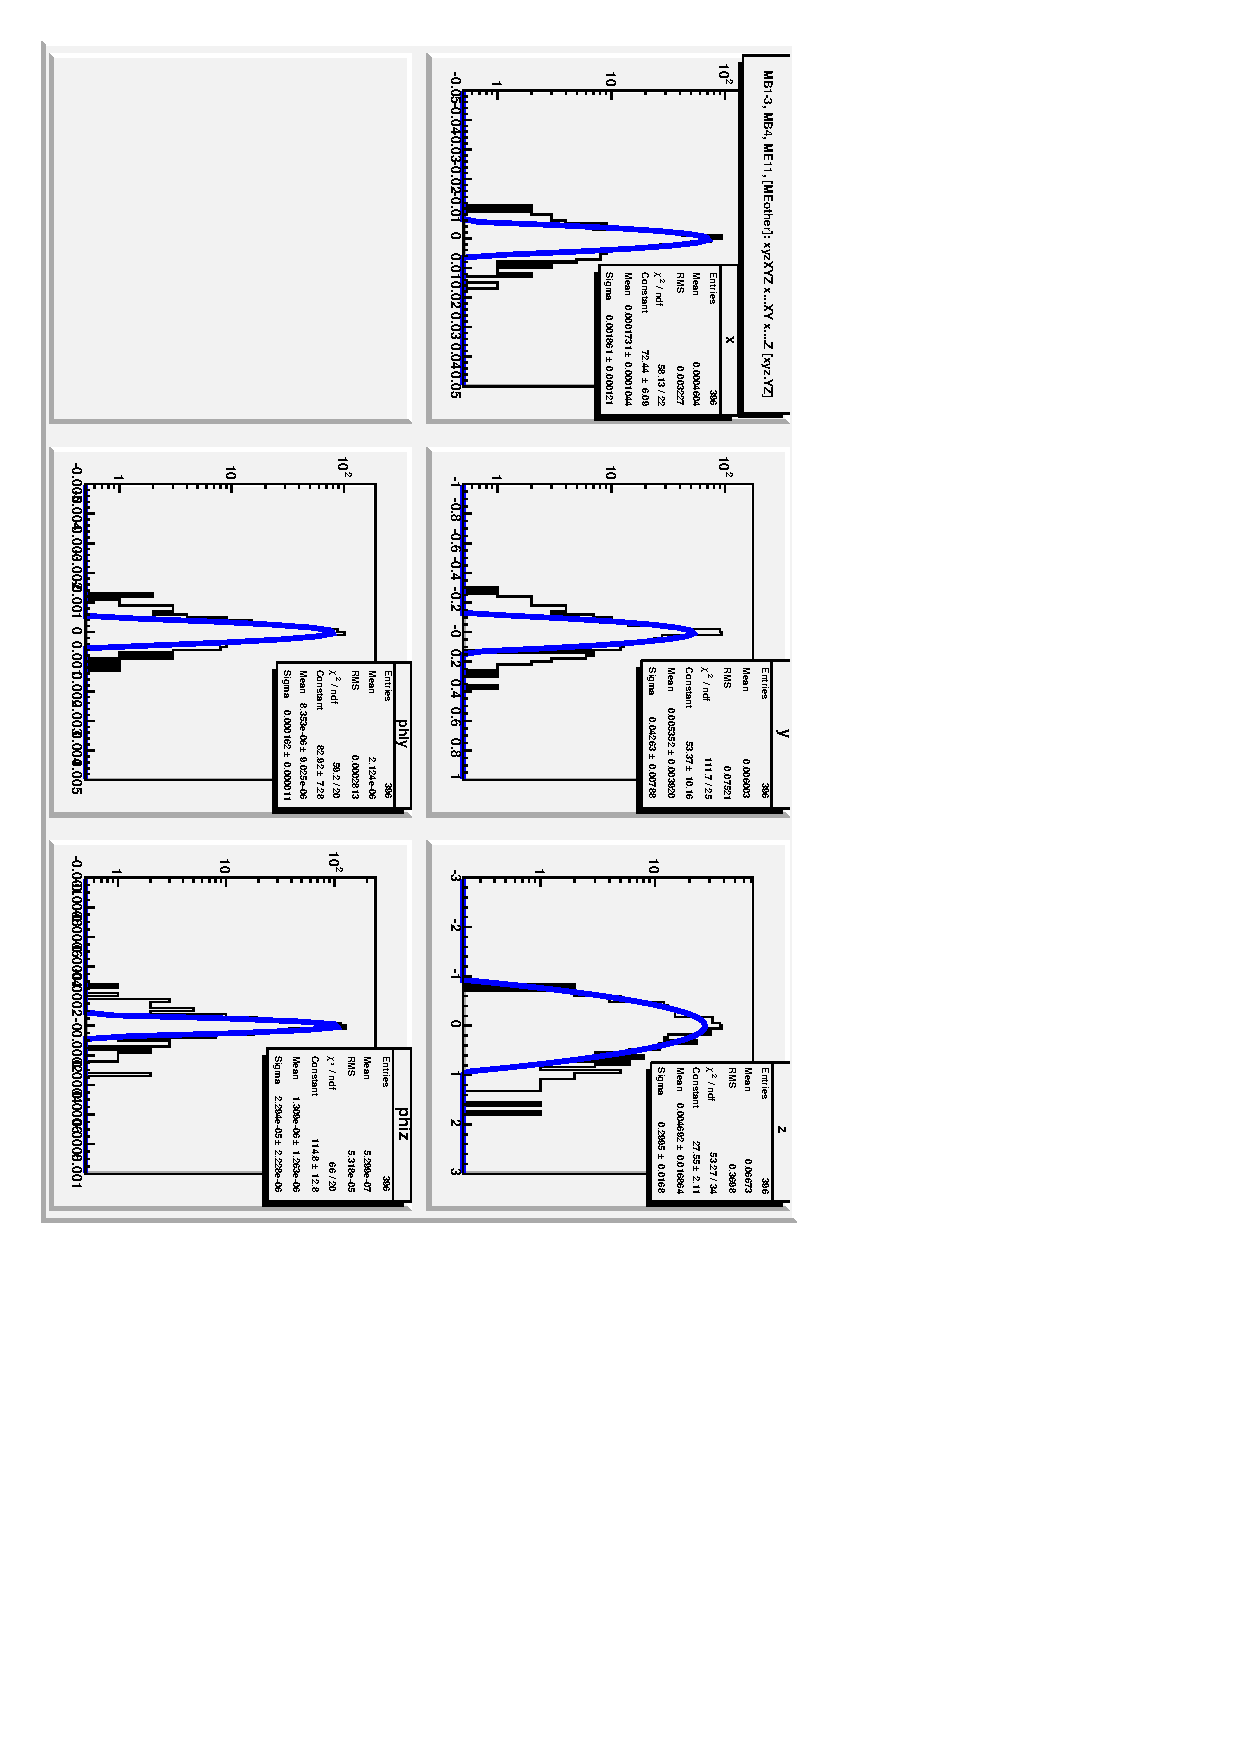
\includegraphics[height=0.7\linewidth, angle=90]{optimal_endcap_alignment.pdf}
\end{center}

\vspace{-0.75 cm}
\begin{columns}
\column{0.5\linewidth}
\begin{center}
All but ME1/1
\begin{tabular}{c c | c c}
\hline\hline
$x$ & 19 $\mu$m & \\
$y$ & 430 $\mu$m & 0.16 mrad & $\phi_y$ \\
$z$ & 3.0 mm & 0.03 mrad & $\phi_z$ \\
\hline\hline
\end{tabular}
\end{center}

\column{0.5\linewidth}
\begin{center}
ME 1/1: possible software bug
\begin{tabular}{c c}
\hline\hline
$x$ & 300 $\mu$m \\
$y$ & 2--6 mm asymmetry \\
angles & 1 mrad or more \\
\hline\hline
\end{tabular}
\end{center}
\end{columns}
\end{frame}

\begin{frame}
\frametitle{Dependence on integrated luminosity: accuracy}
%% \begin{itemize}
%% \item Resolution of some parameters improves with statistics, \\
%% others reach a limit (``brick wall'') due to systematic effects
%% \end{itemize}

%% \vspace{-0.5 cm}
%% \begin{columns}
%% \column{0.5\linewidth}
%% \begin{center}
%% Barrel brick walls (pb$^{-1}$)
%% \begin{tabular}{c c | c c}
%% \hline $x$ & $>$80 & 15 & $\phi_x$ \\
%% $y$ & 3 & 20 & $\phi_y$ \\
%% \mbox{\hspace{0.2 cm}} $z$ \mbox{\hspace{0.2 cm}} & 3 & 20 & \mbox{\hspace{0.2 cm}} $\phi_z$ \mbox{\hspace{0.2 cm}} \\
%% \end{tabular}
%% \end{center}
%% \column{0.5\linewidth}
%% \begin{center}
%% Endcap brick walls (pb$^{-1}$)
%% \begin{tabular}{c c | c c}
%% \hline $x$ & $>$80 & & \\
%% $y$ & $>$80 & $>$80 & $\phi_y$ \\
%% \mbox{\hspace{0.2 cm}} $z$ \mbox{\hspace{0.2 cm}} & 30 & $>$80 & \mbox{\hspace{0.2 cm}} $\phi_z$ \mbox{\hspace{0.2 cm}} \\
%% \end{tabular}
%% \end{center}
%% \end{columns}

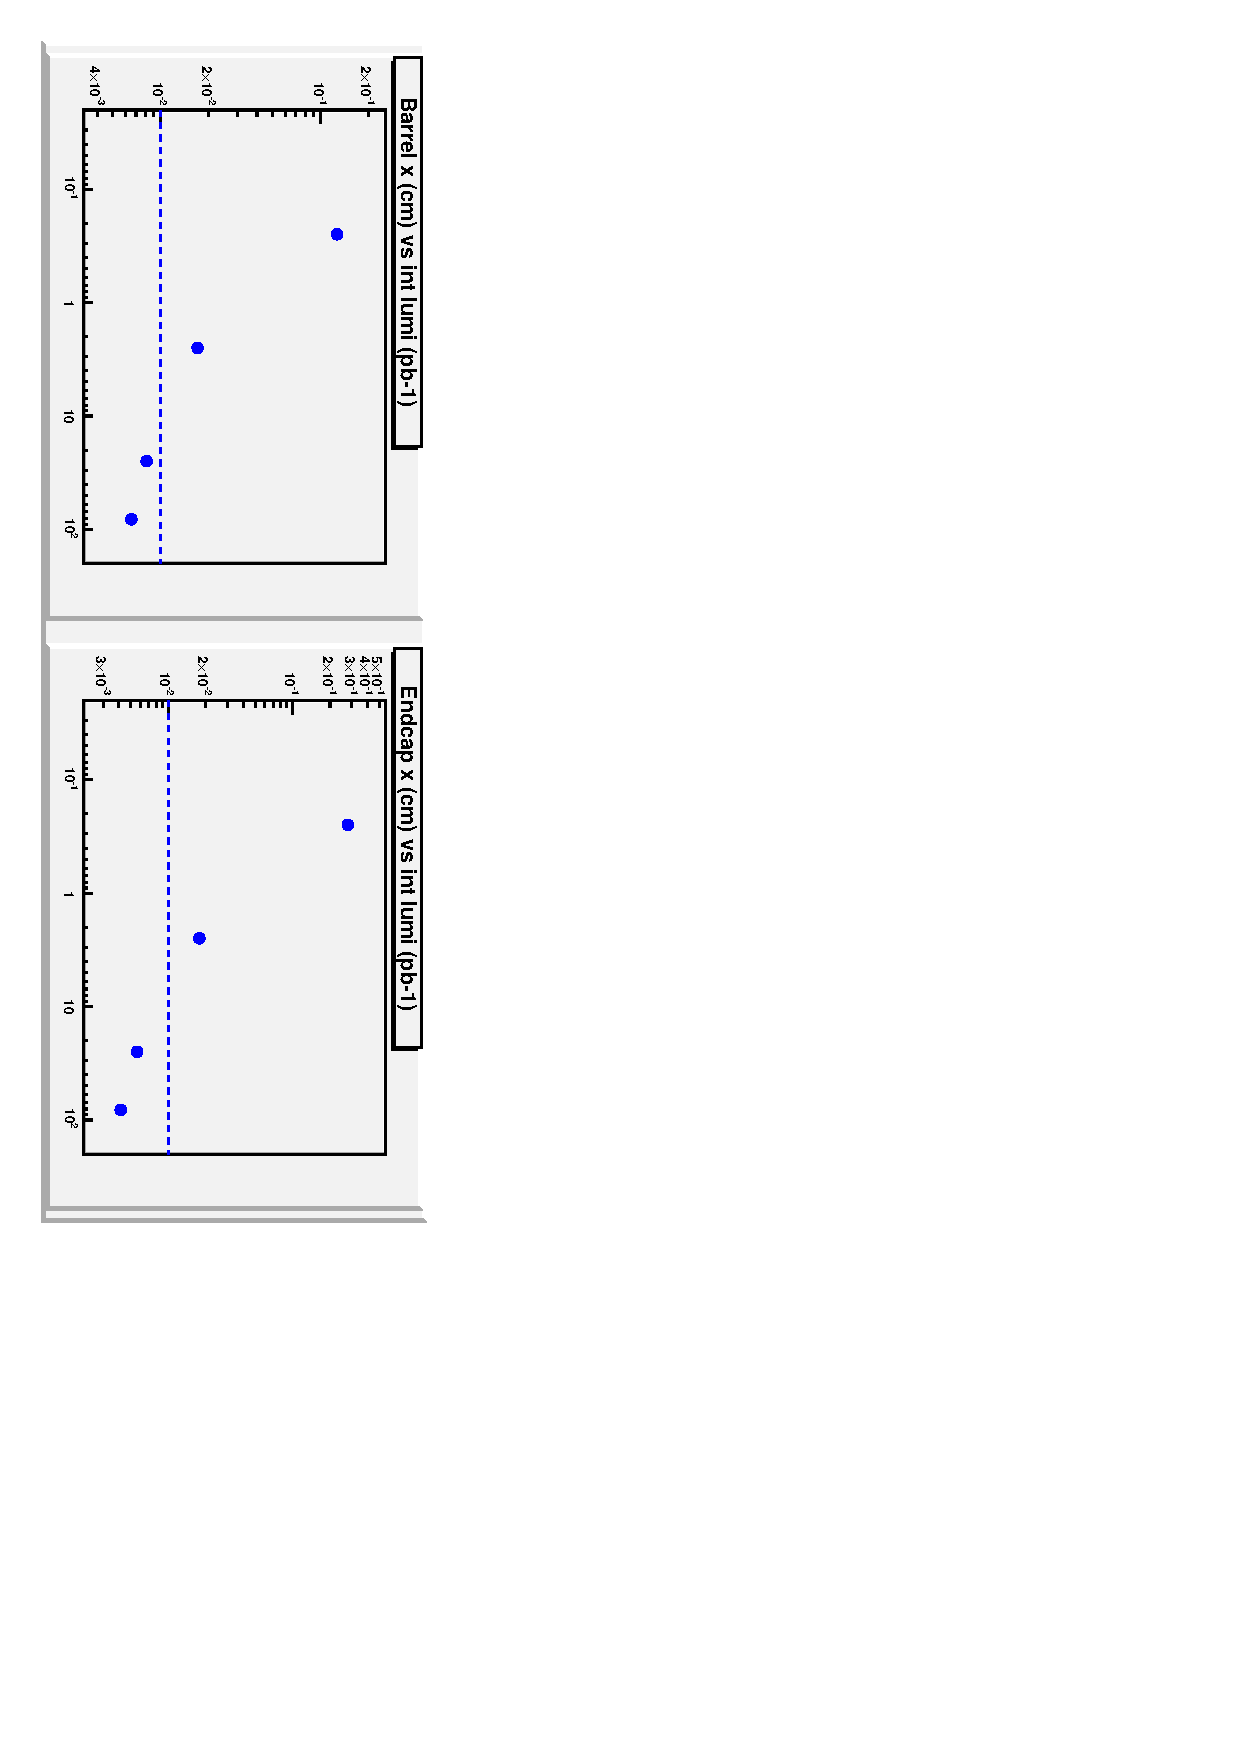
\includegraphics[height=\linewidth, angle=90]{events_x_wacky.pdf}

%% \begin{center}
%% \only<1>{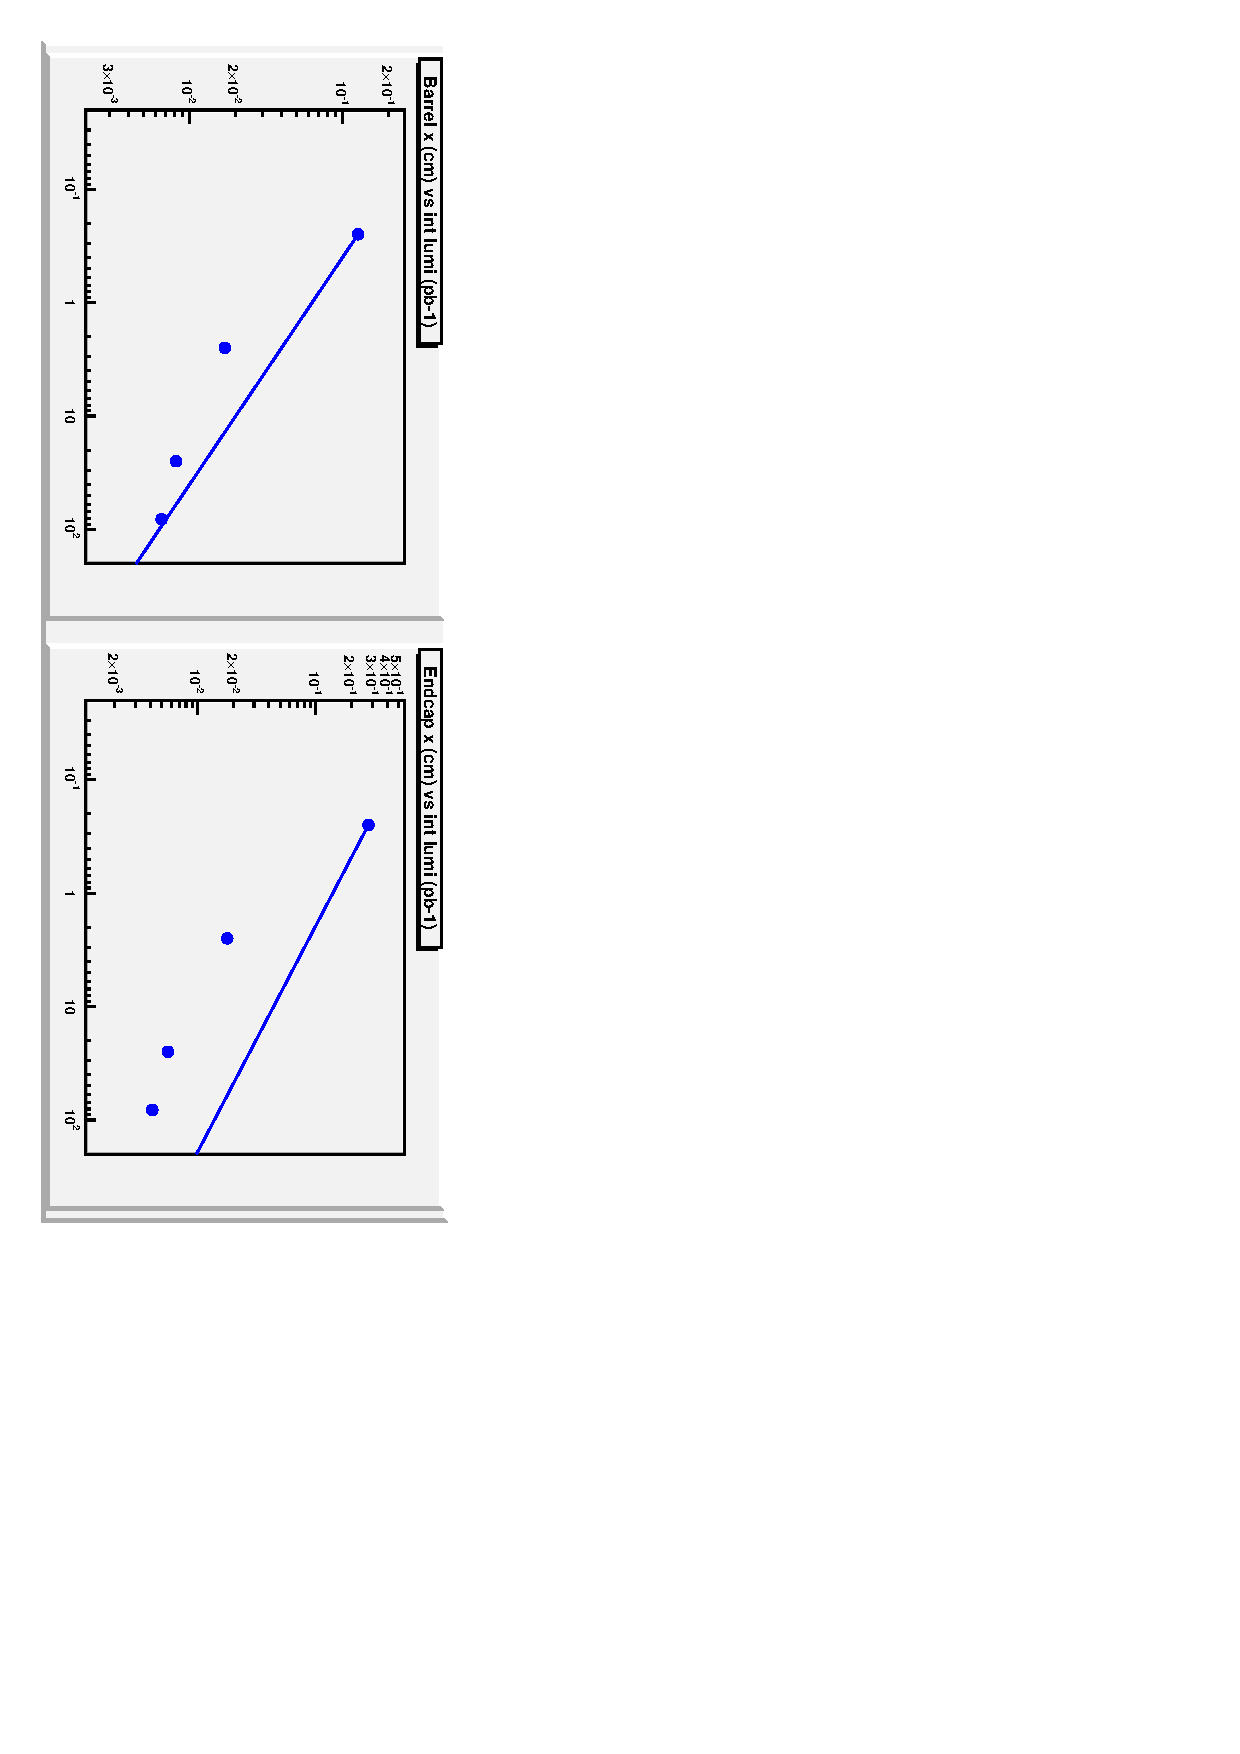
\includegraphics[height=0.85\linewidth, angle=90]{events_x_rmsonly.pdf}

%% 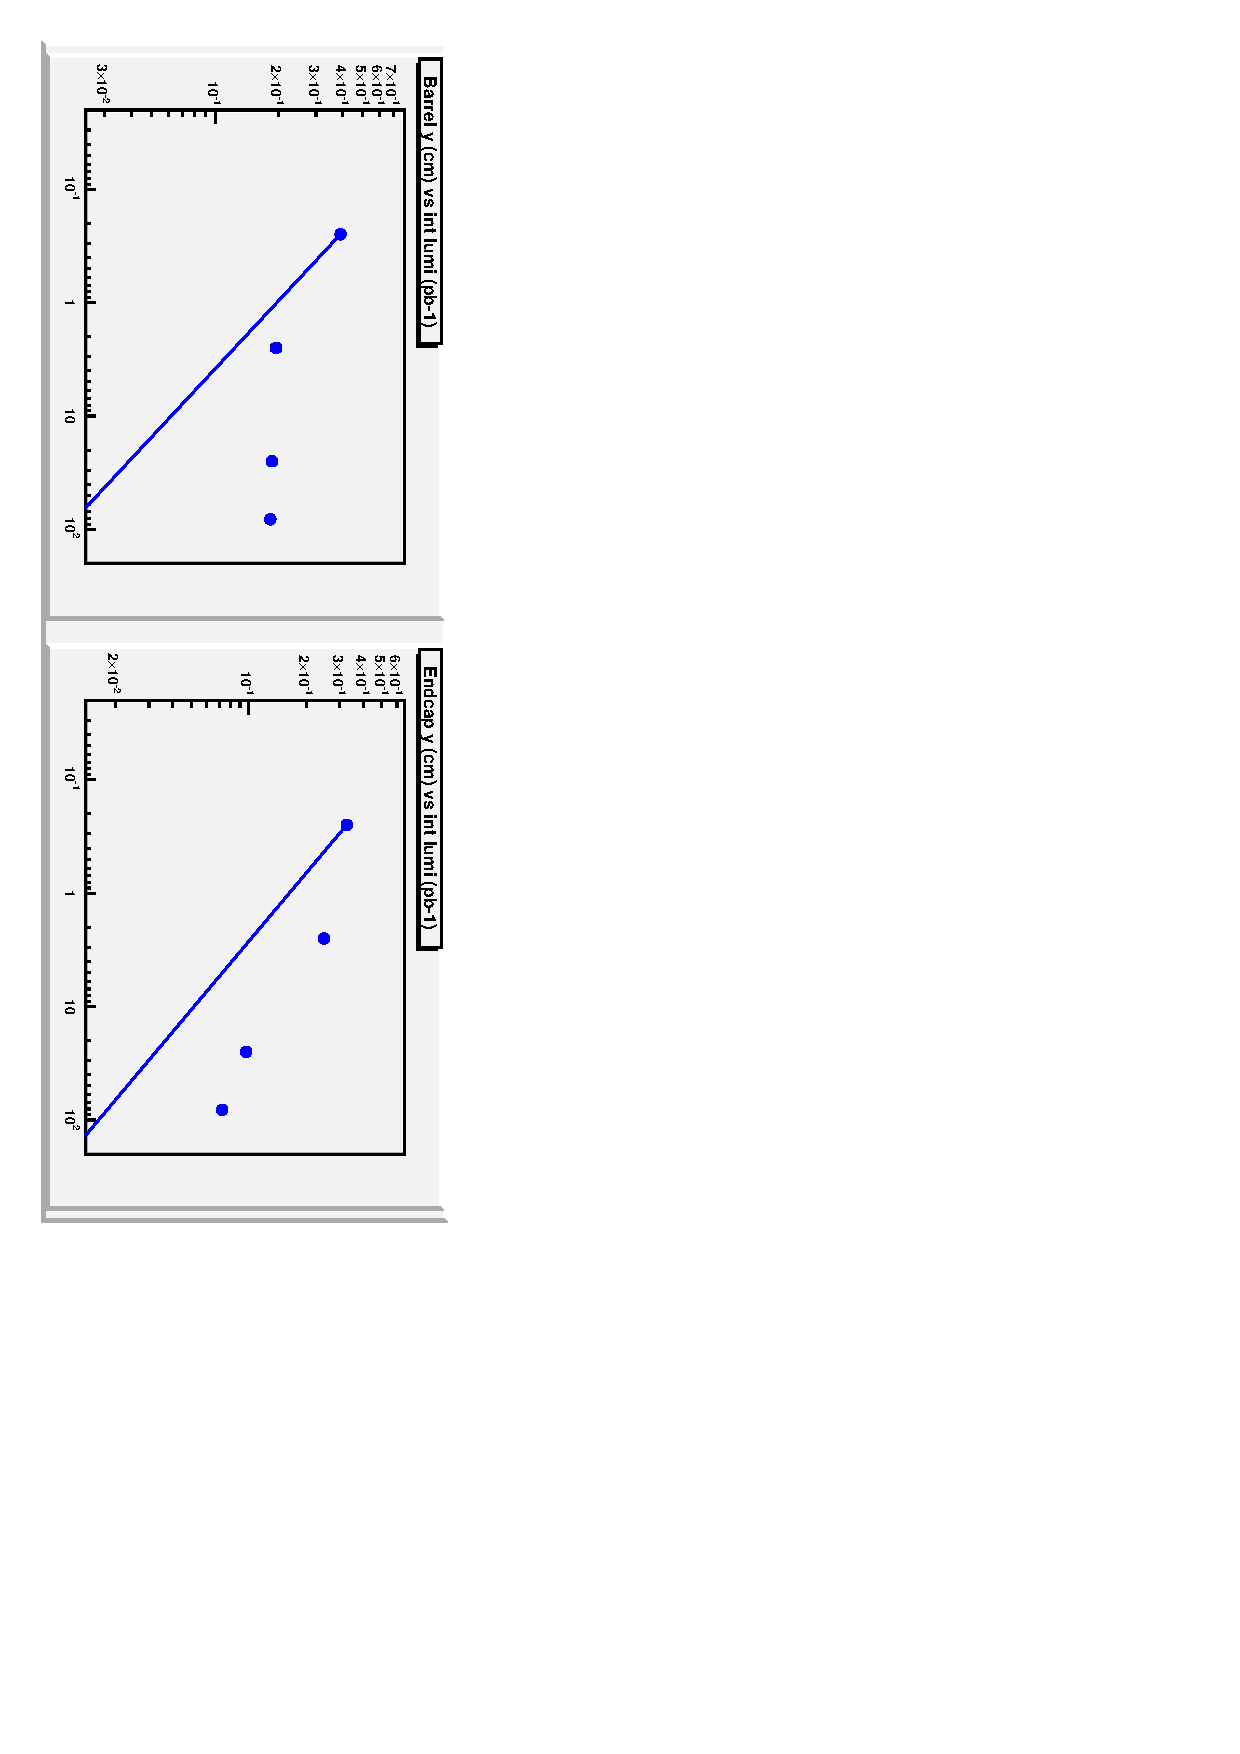
\includegraphics[height=0.85\linewidth, angle=90]{events_y_rmsonly.pdf}}
%% \only<2>{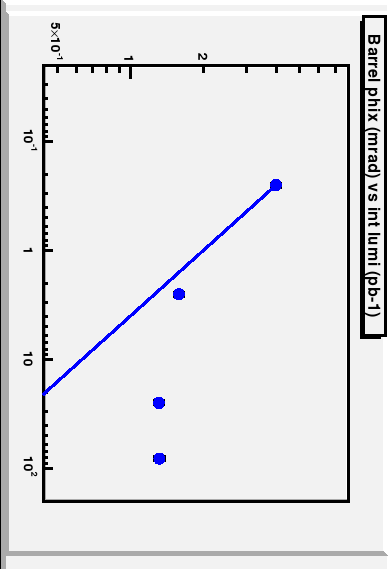
\includegraphics[height=0.425\linewidth, angle=90]{events_phix_rmsonly.png}\mbox{\hspace{0.425\linewidth}}

%% 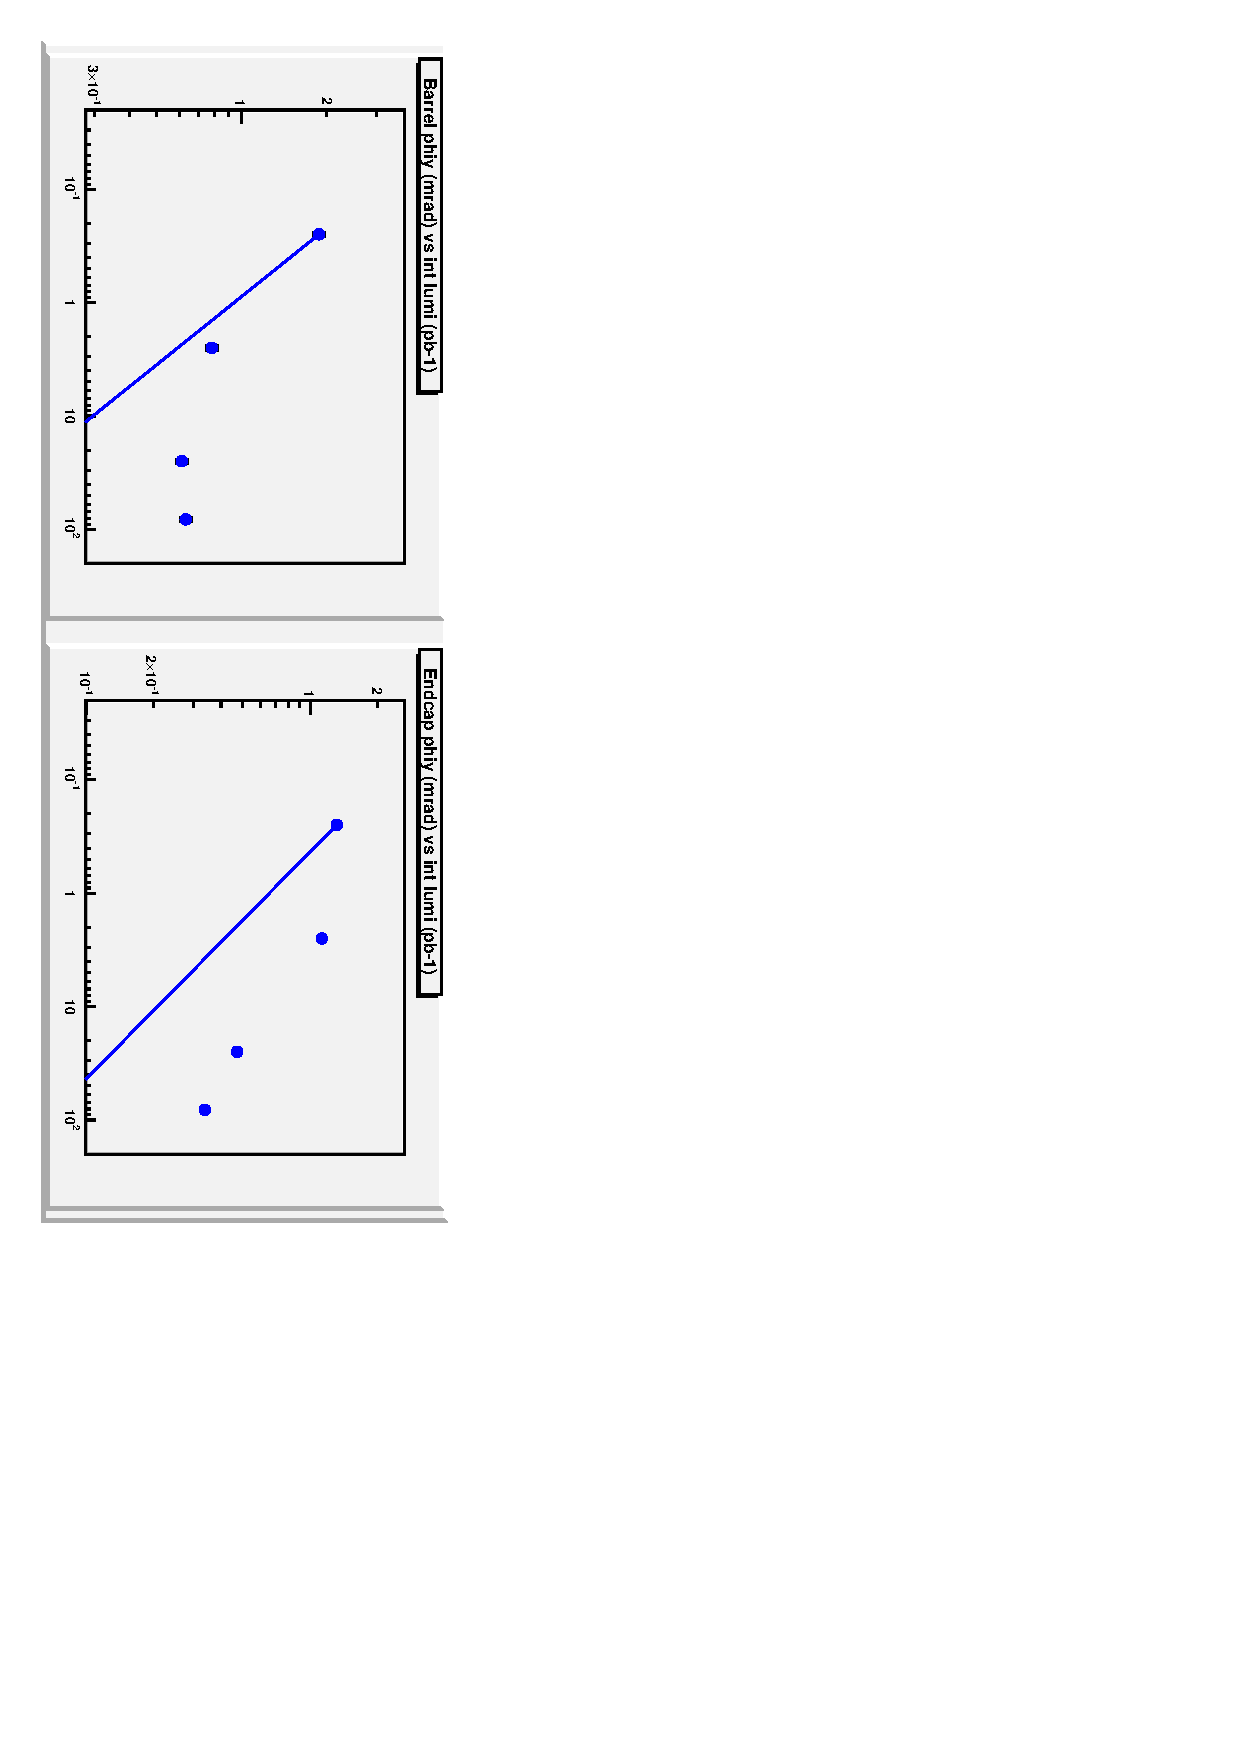
\includegraphics[height=0.85\linewidth, angle=90]{events_phiy_rmsonly.pdf}}
%% \only<3>{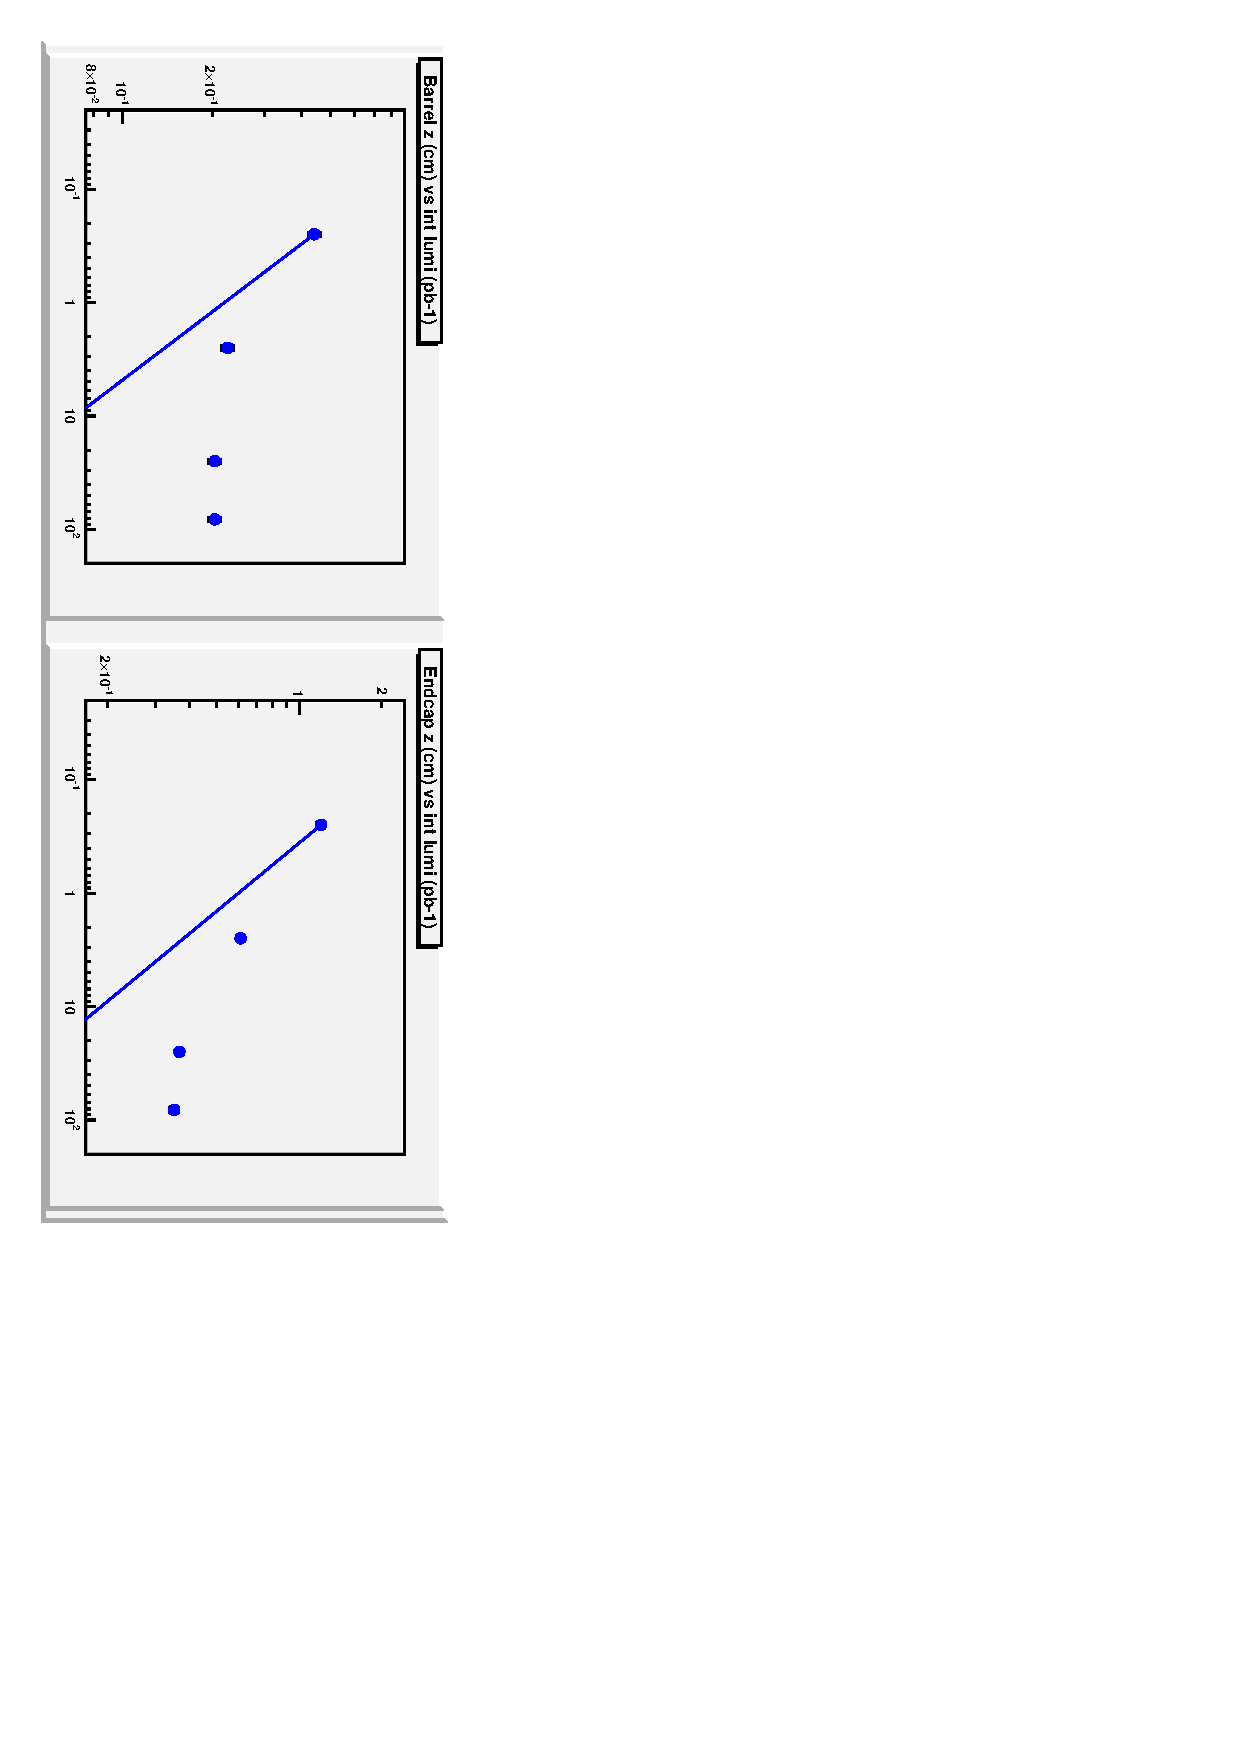
\includegraphics[height=0.85\linewidth, angle=90]{events_z_rmsonly.pdf}

%% 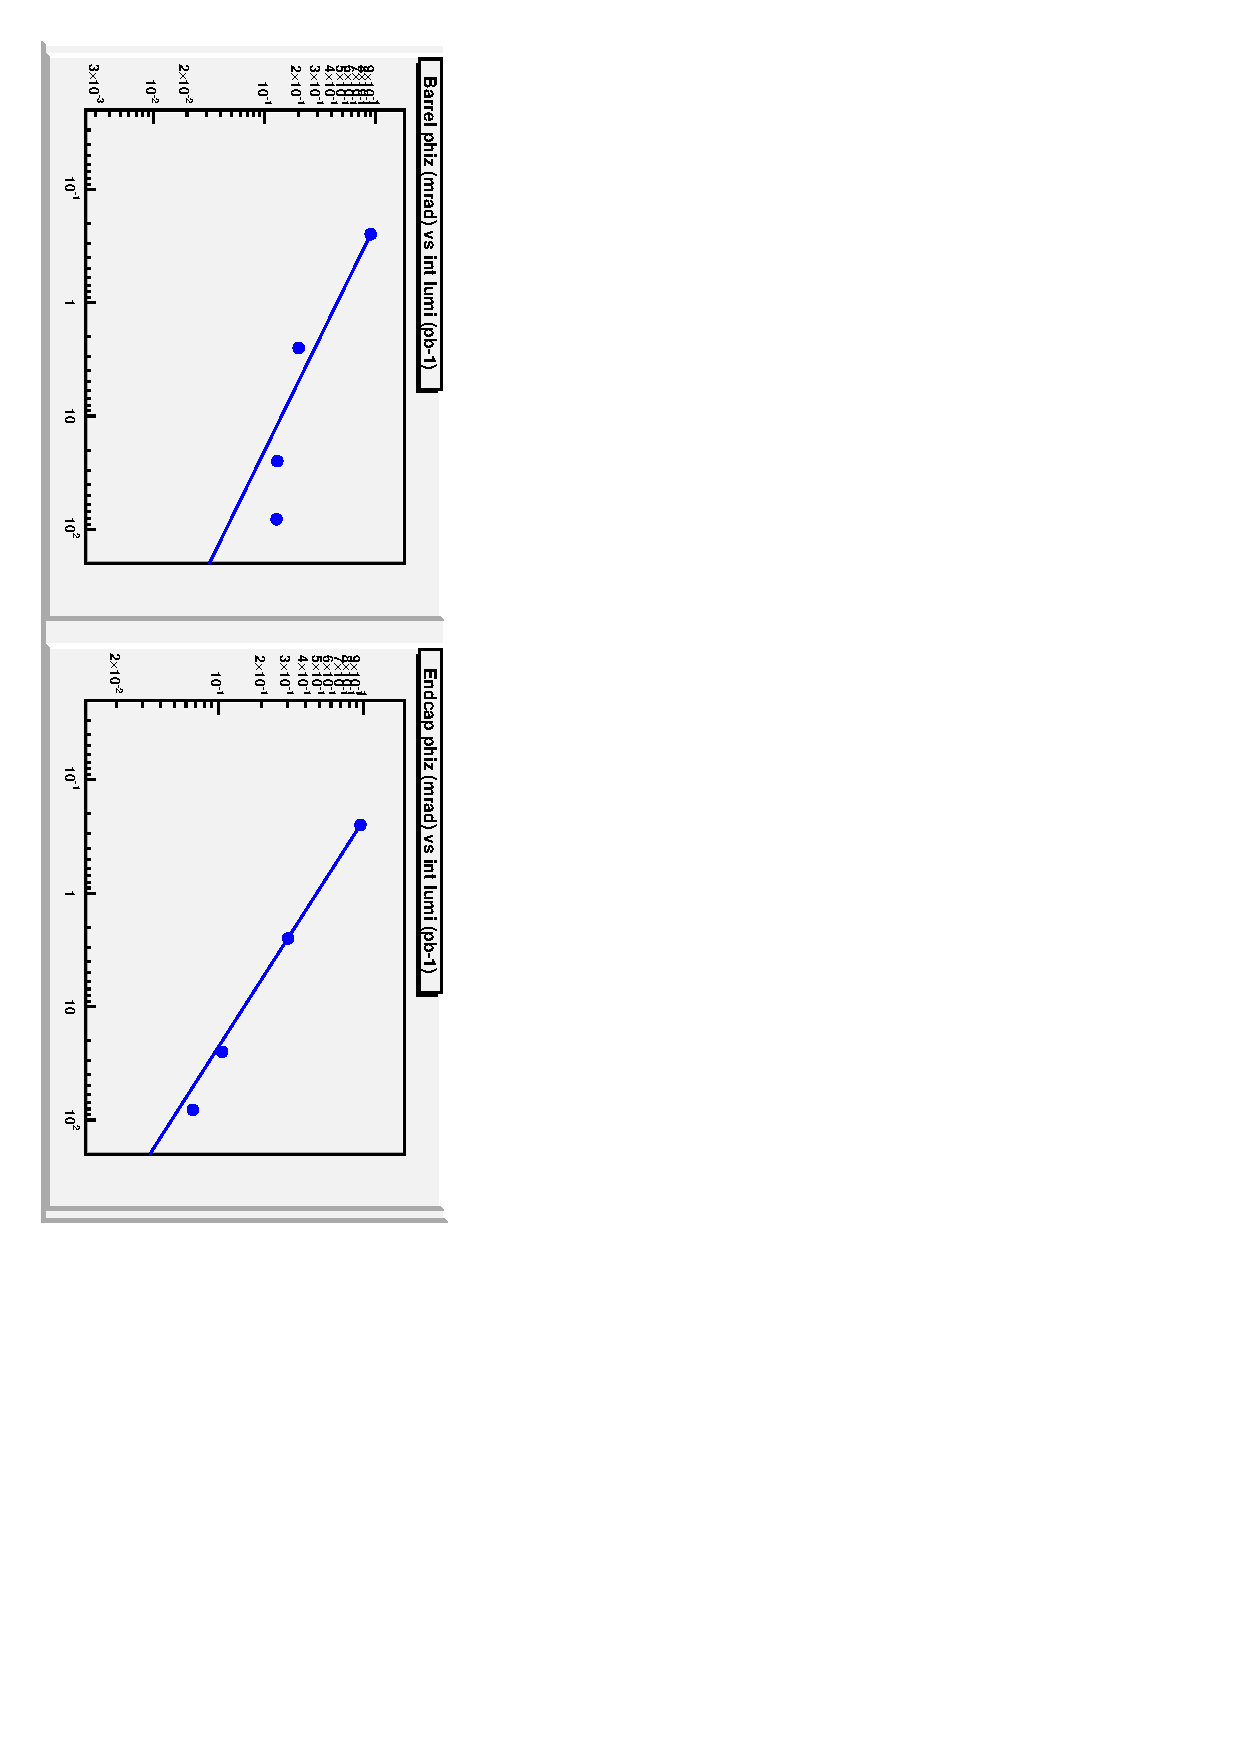
\includegraphics[height=0.85\linewidth, angle=90]{events_phiz_rmsonly.pdf}}
%% \end{center}

\vspace{0.25 cm}
\begin{itemize}\setlength{\itemsep}{0.25 cm}
\item Points: RMS of distribution, Line: 100~$\mu$m
\item $x$ accuracy reaches 100~$\mu$m with 10~pb$^{-1}$
\end{itemize}

\end{frame}

\begin{frame}
\frametitle{Dependence on integrated luminosity: $Z$, $Z'$ resolution}
\vspace{0.25 cm}
\begin{columns}
\column{0.5\linewidth}
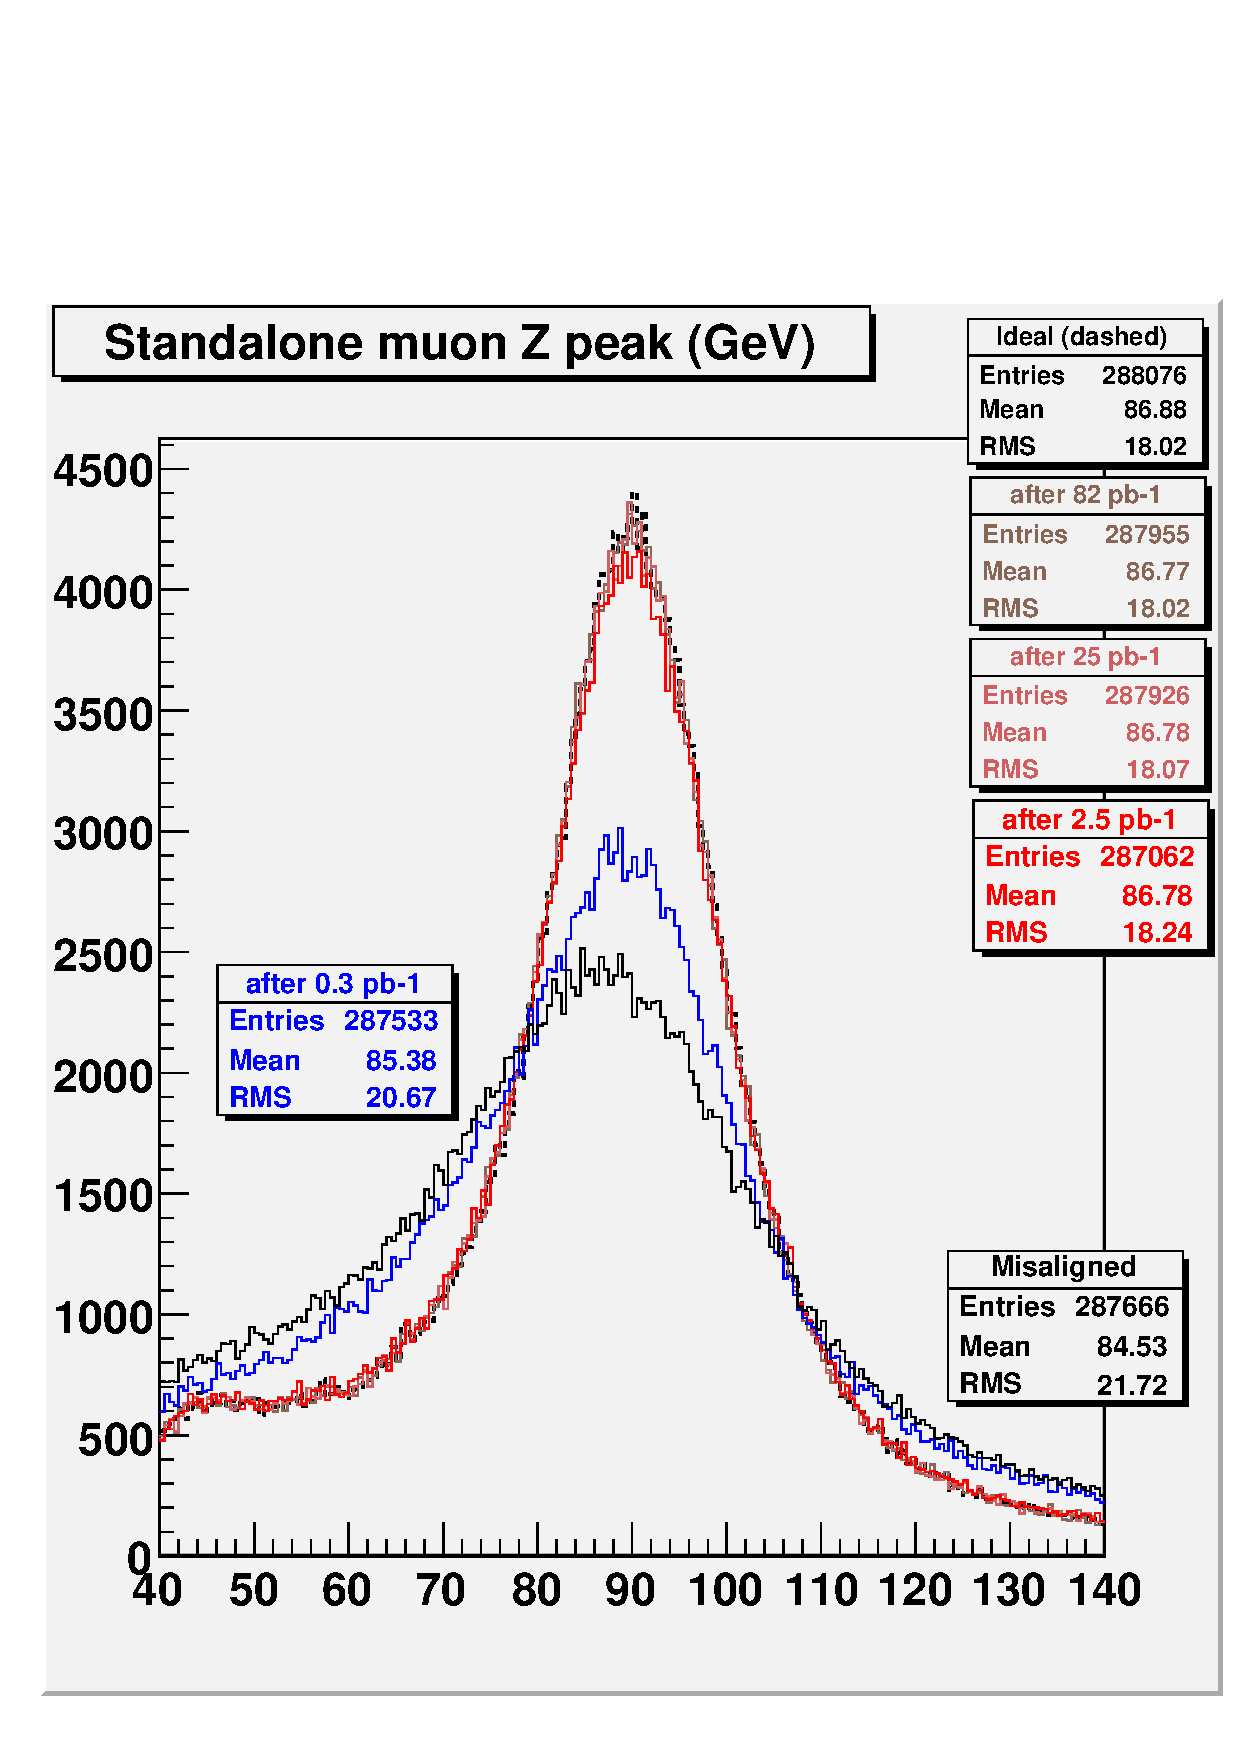
\includegraphics[width=\linewidth]{checkit_standaloneZ.pdf}
\column{0.5\linewidth}
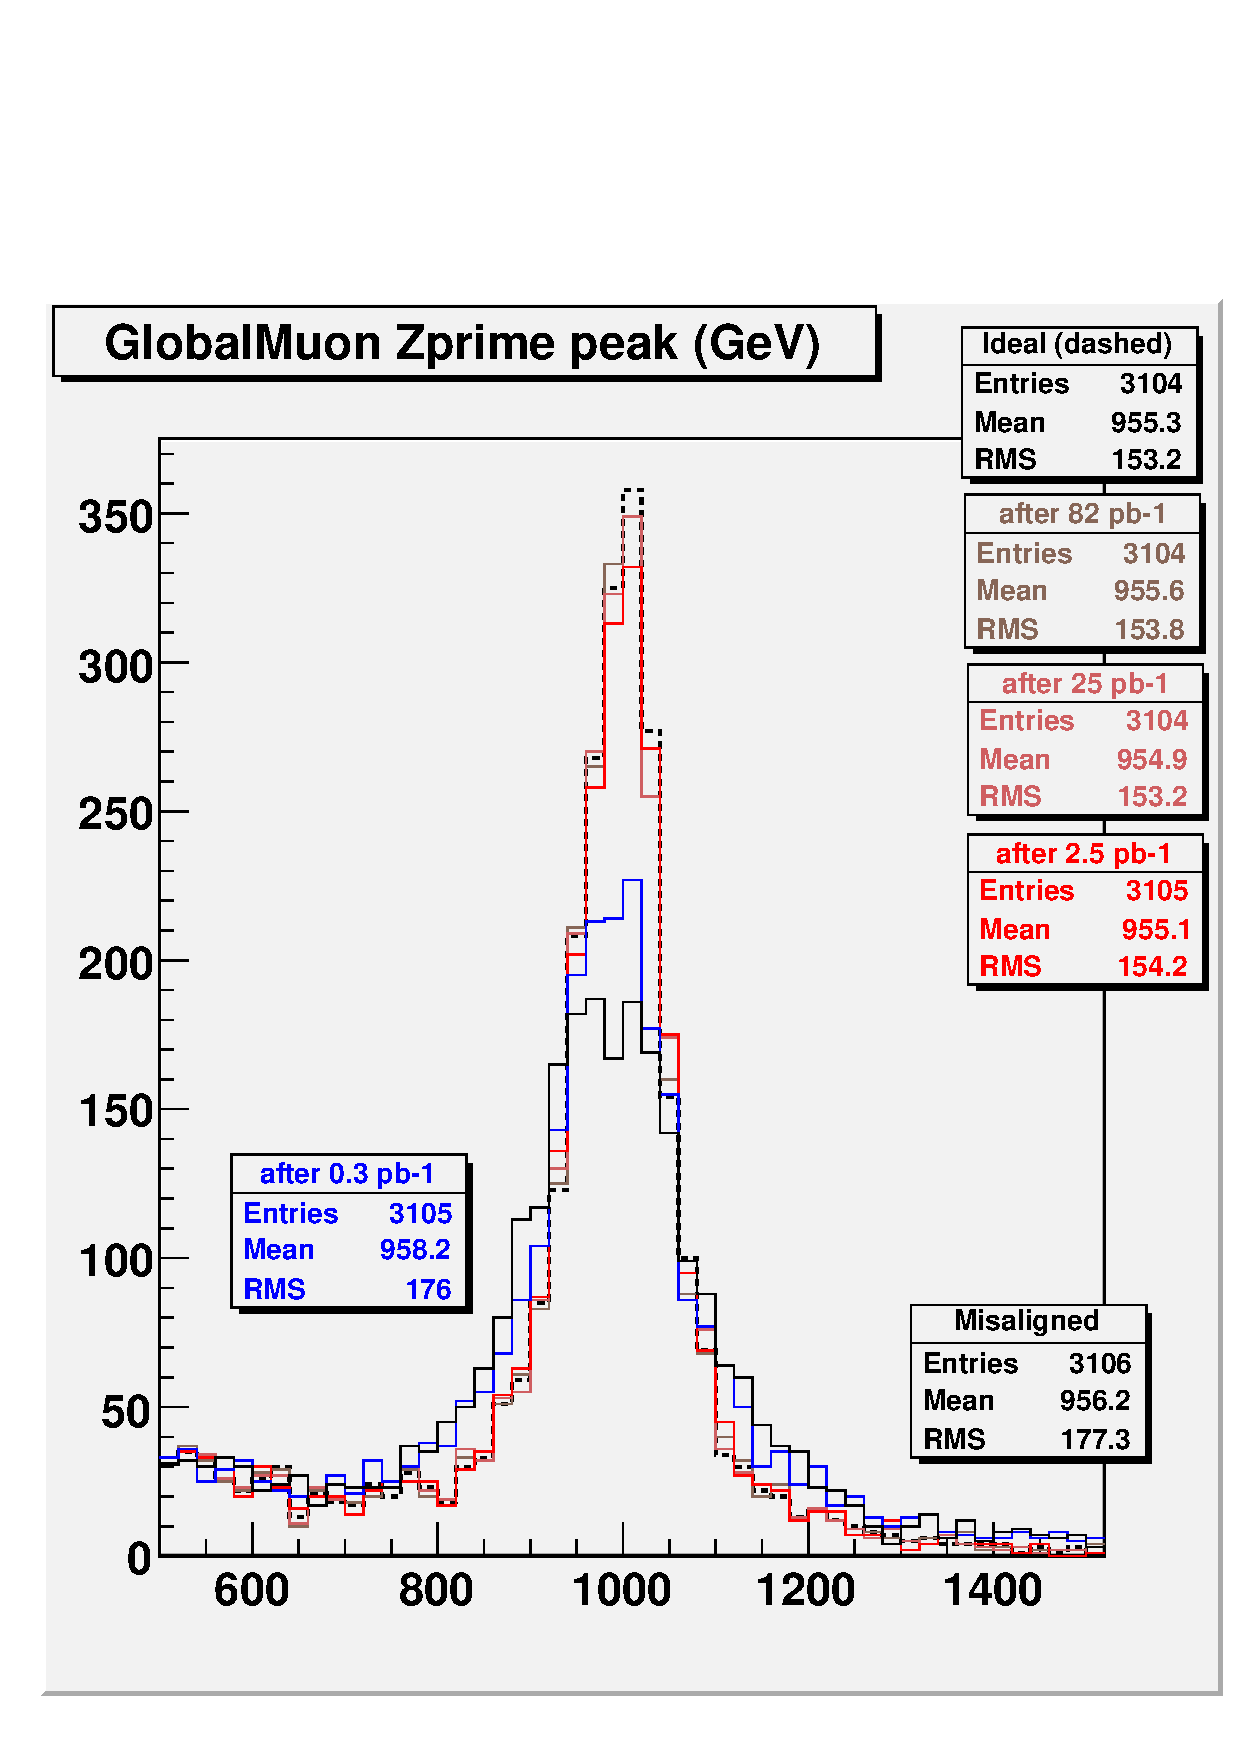
\includegraphics[width=\linewidth]{checkit_globZprime.pdf}
\end{columns}

\vspace{0.25 cm}
\begin{itemize}
\item To do: higher moments of distribution--- Drell-Yan smearing
\end{itemize}
\vspace{-0.25 cm}
\mbox{ }
\end{frame}

\begin{frame}
\frametitle{CSC layer-by-layer alignment}
\begin{itemize}
\item CSC layers known to be misaligned (Karoly, Andrey, Oleg\ldots)
\end{itemize}
\begin{center}
\begin{tabular}{c c c}
& current (RMS) & after 82~pb$^{-1}$ alignment (RMS) \\\hline
$x$ & 190 $\mu$m & 38 $\mu$m \\
$y$ & 340 $\mu$m & 860 $\mu$m \\
$\phi_z$ & 0.04 mrad & 0.06 mrad \\
\end{tabular}
\end{center}
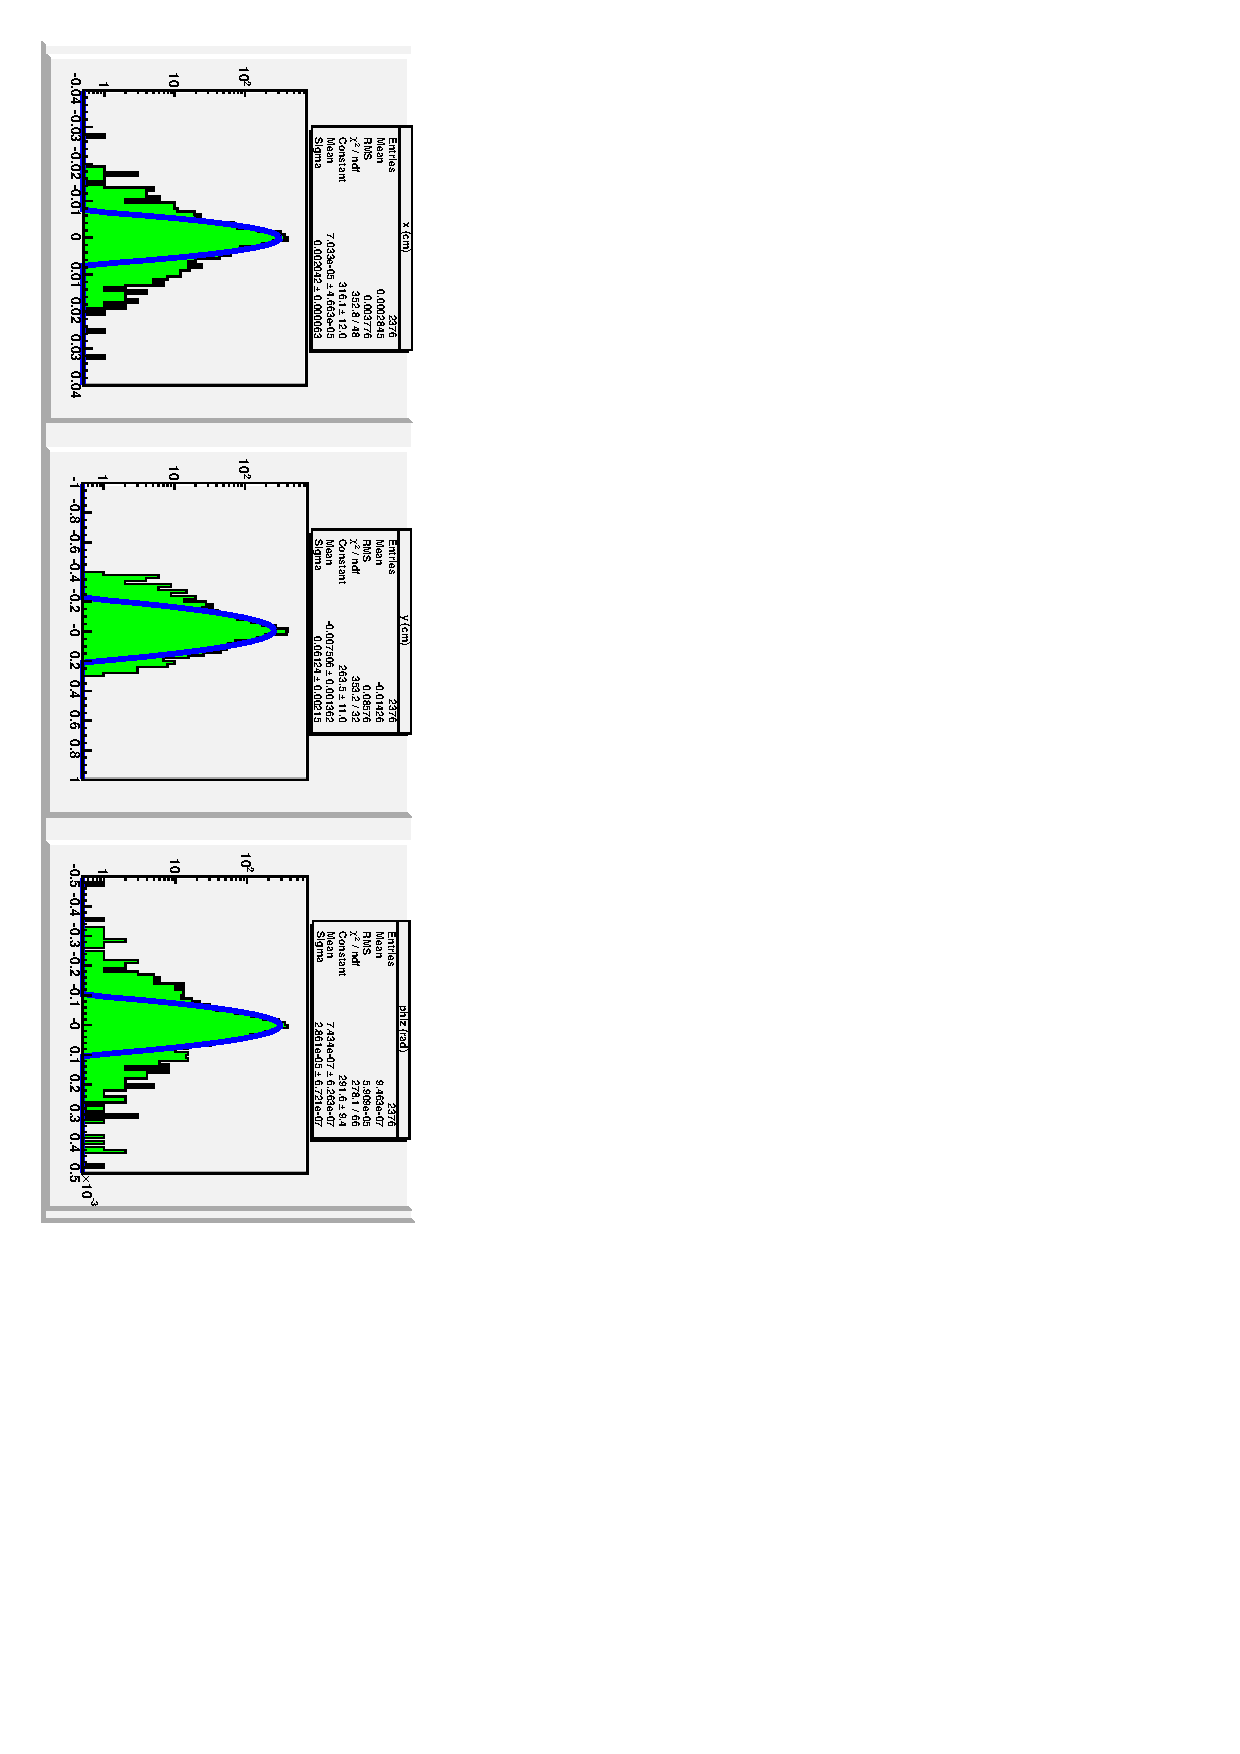
\includegraphics[height=\linewidth, angle=90]{layer_alignment.pdf}
\end{frame}

\section*{Systematics studies}

\begin{frame}
\begin{center}
\Huge \textcolor{blue}{Systematics studies}
\end{center}
\end{frame}

\begin{frame}
\frametitle{Effect of tracker misalignment (1 of 3)}
\begin{itemize}
\item Wheel/disk procedure: becomes significant when tracker is
misaligned 2--3 times worse than ``short-term scenario''

\begin{center}
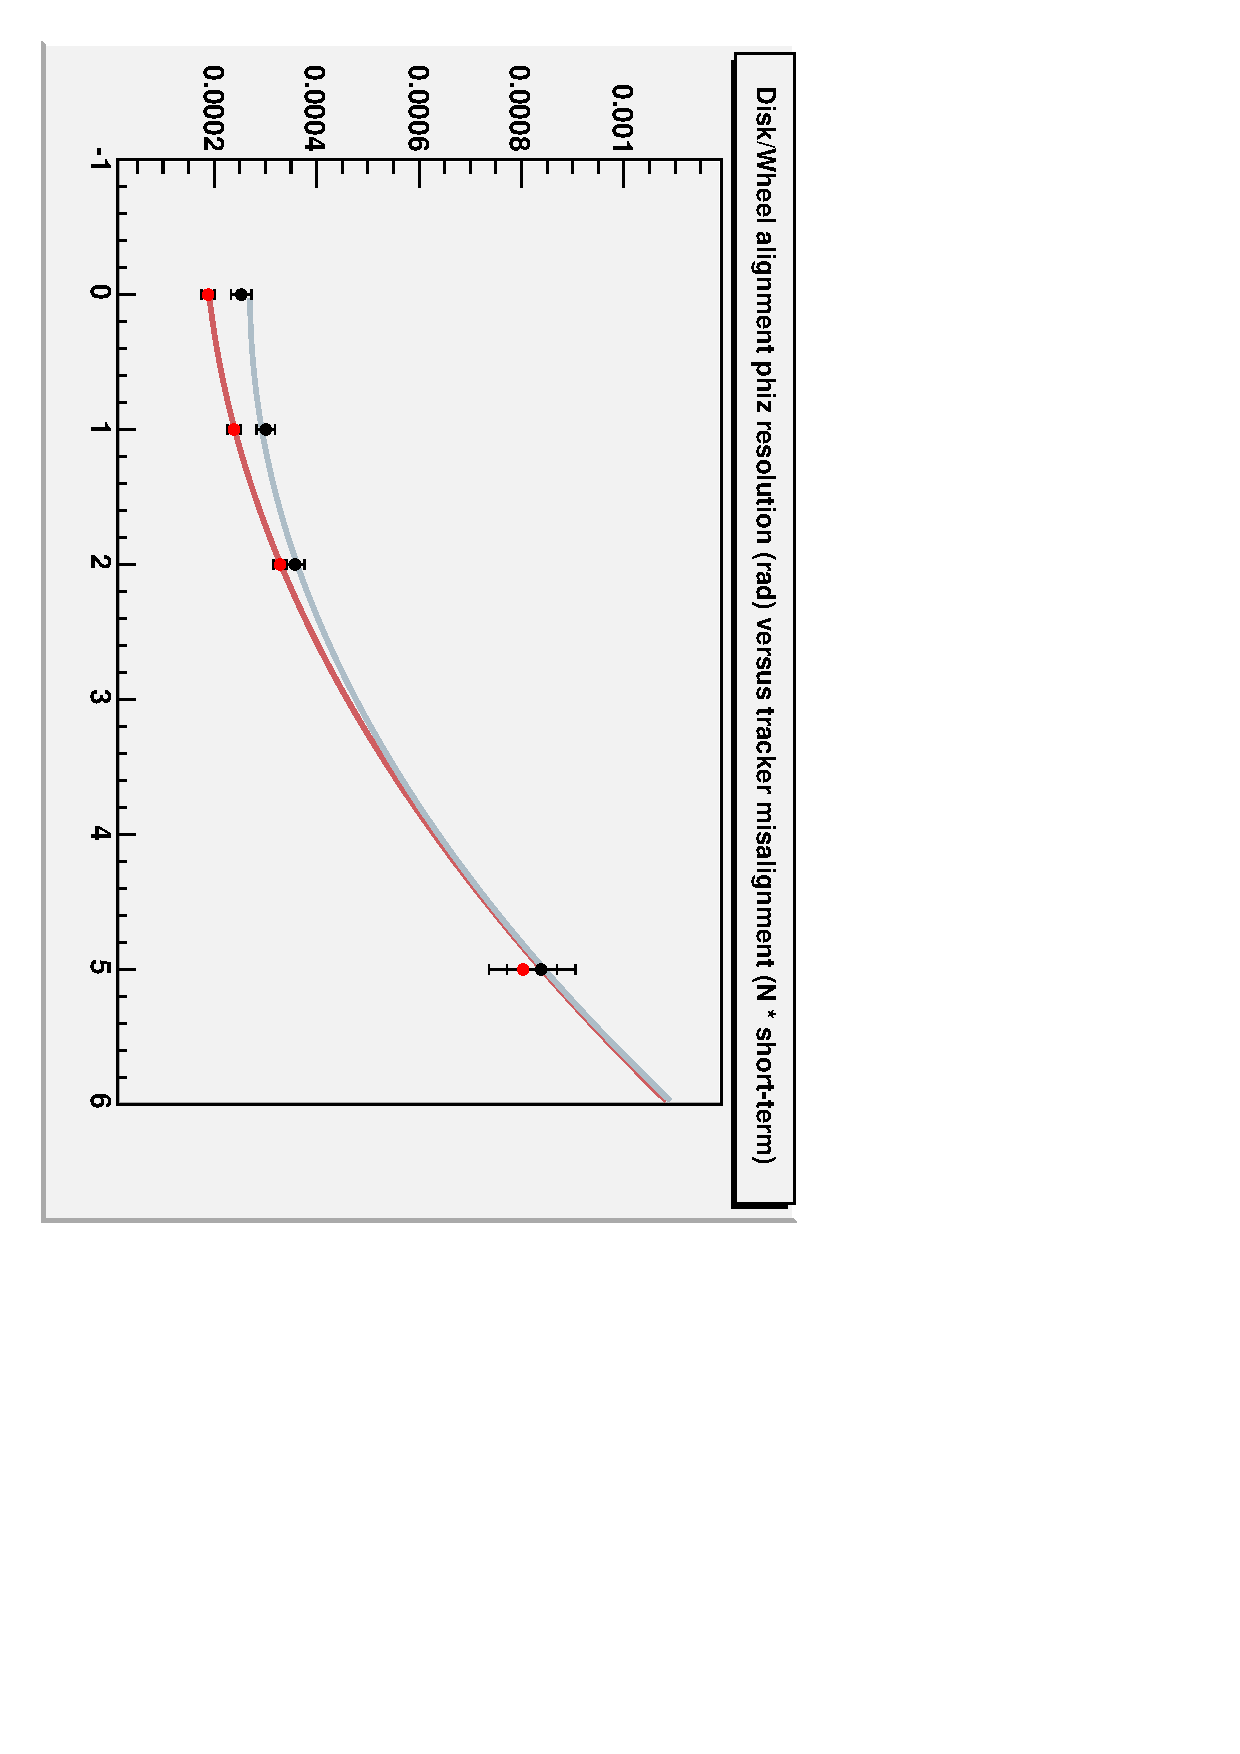
\includegraphics[height=0.8\linewidth, angle=90]{vstracker_disk.pdf}
\end{center}

\item Black: wheels/disks include large chamber misalignments

Red: chambers are perfectly aligned on wheels/disks
\end{itemize}
\end{frame}

\begin{frame}
\frametitle{Effect of tracker misalignment (2 of 3)}
\begin{itemize}
\item Most sensitive parameters: $x$ and $\phi_z$
\item Accuracy versus $N$ $\times$ tracker ``short-term'' scenario (ST)
\end{itemize}

\begin{columns}
\column{0.8\linewidth}
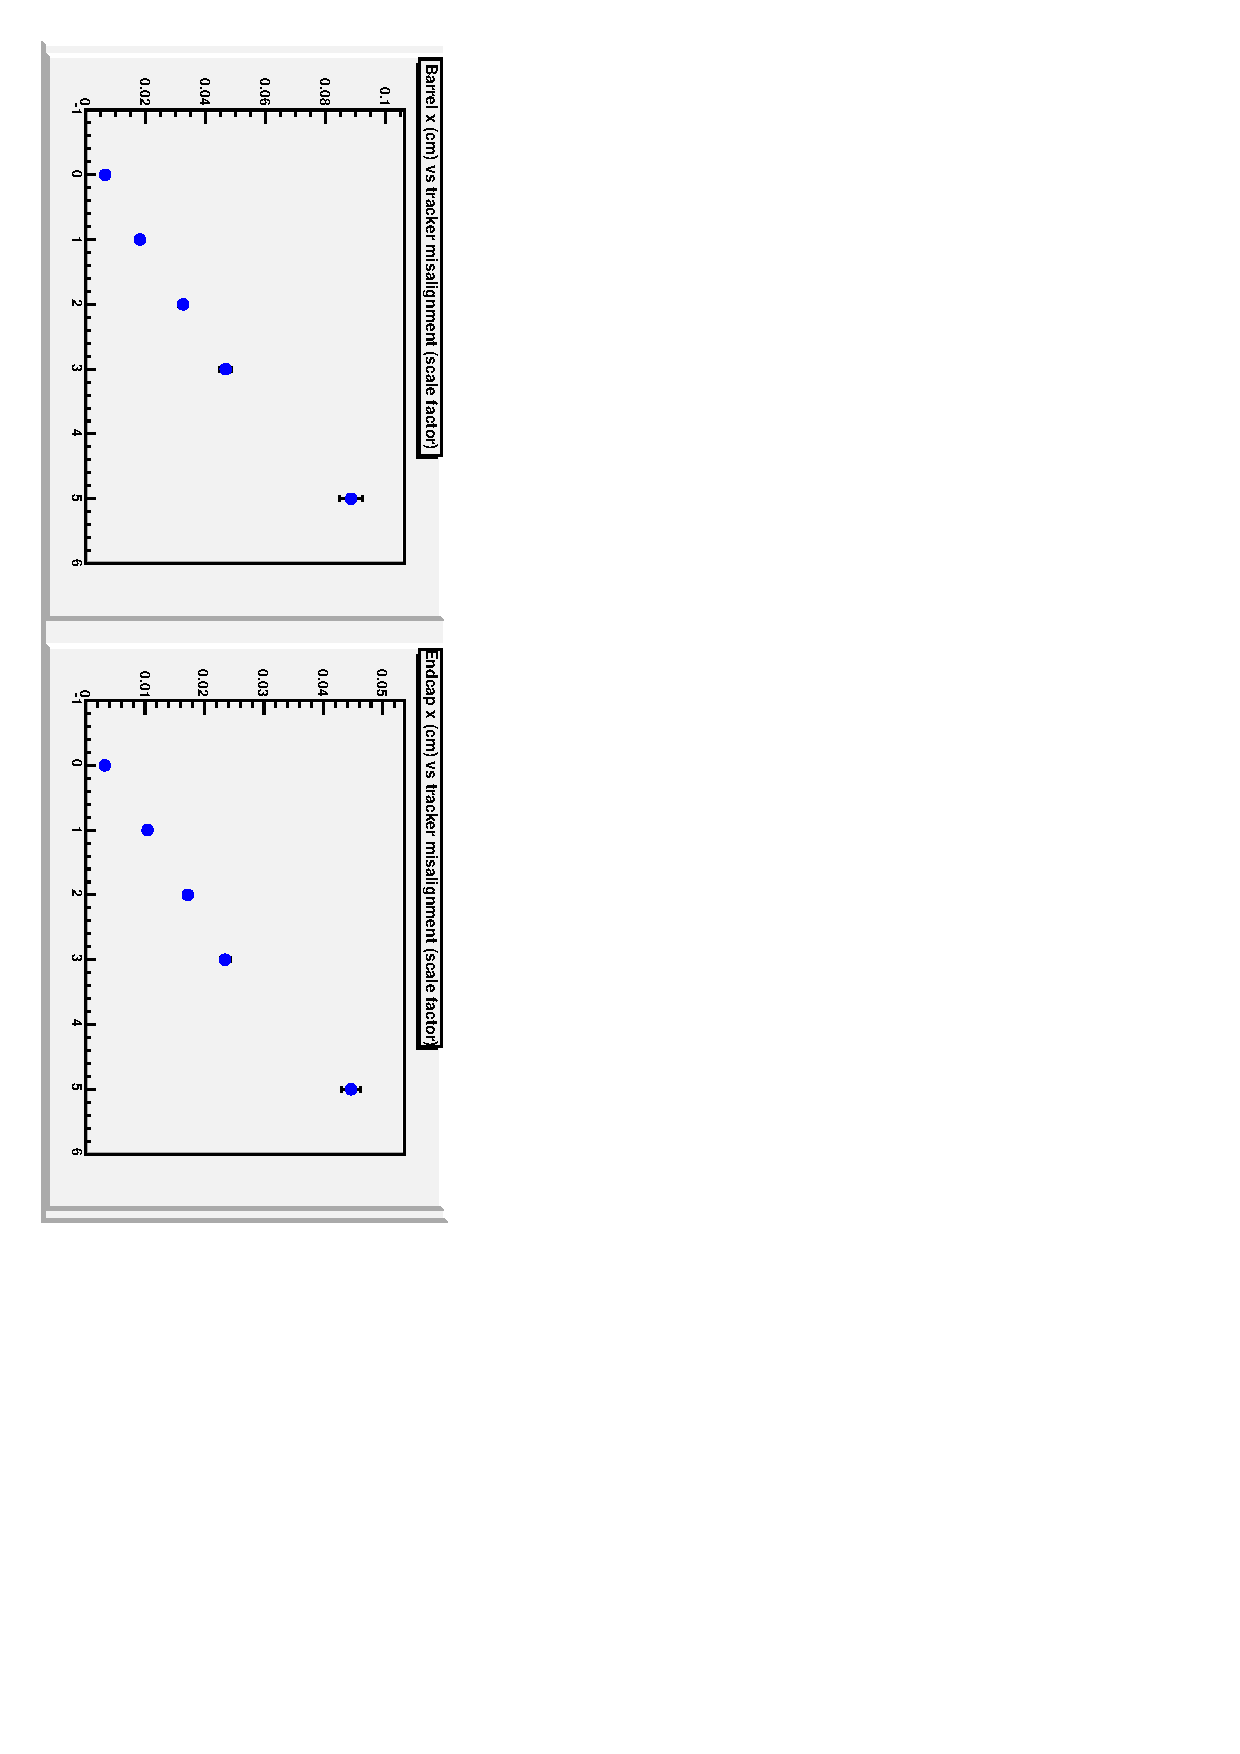
\includegraphics[height=\linewidth, angle=90]{tracker_x_rmsonly.pdf}
\column{0.2\linewidth}
Barrel $x$: 200~$\mu$m/ST

\vspace{0.1 cm}
Endcap $x$: 100~$\mu$m/ST
\end{columns}

\vfill
\begin{columns}
\column{0.2\linewidth}
Barrel $\phi_z$: 0.5~mrad/ST

\vspace{0.1 cm}
Endcap $\phi_z$: 1~mrad/ST

\column{0.8\linewidth}
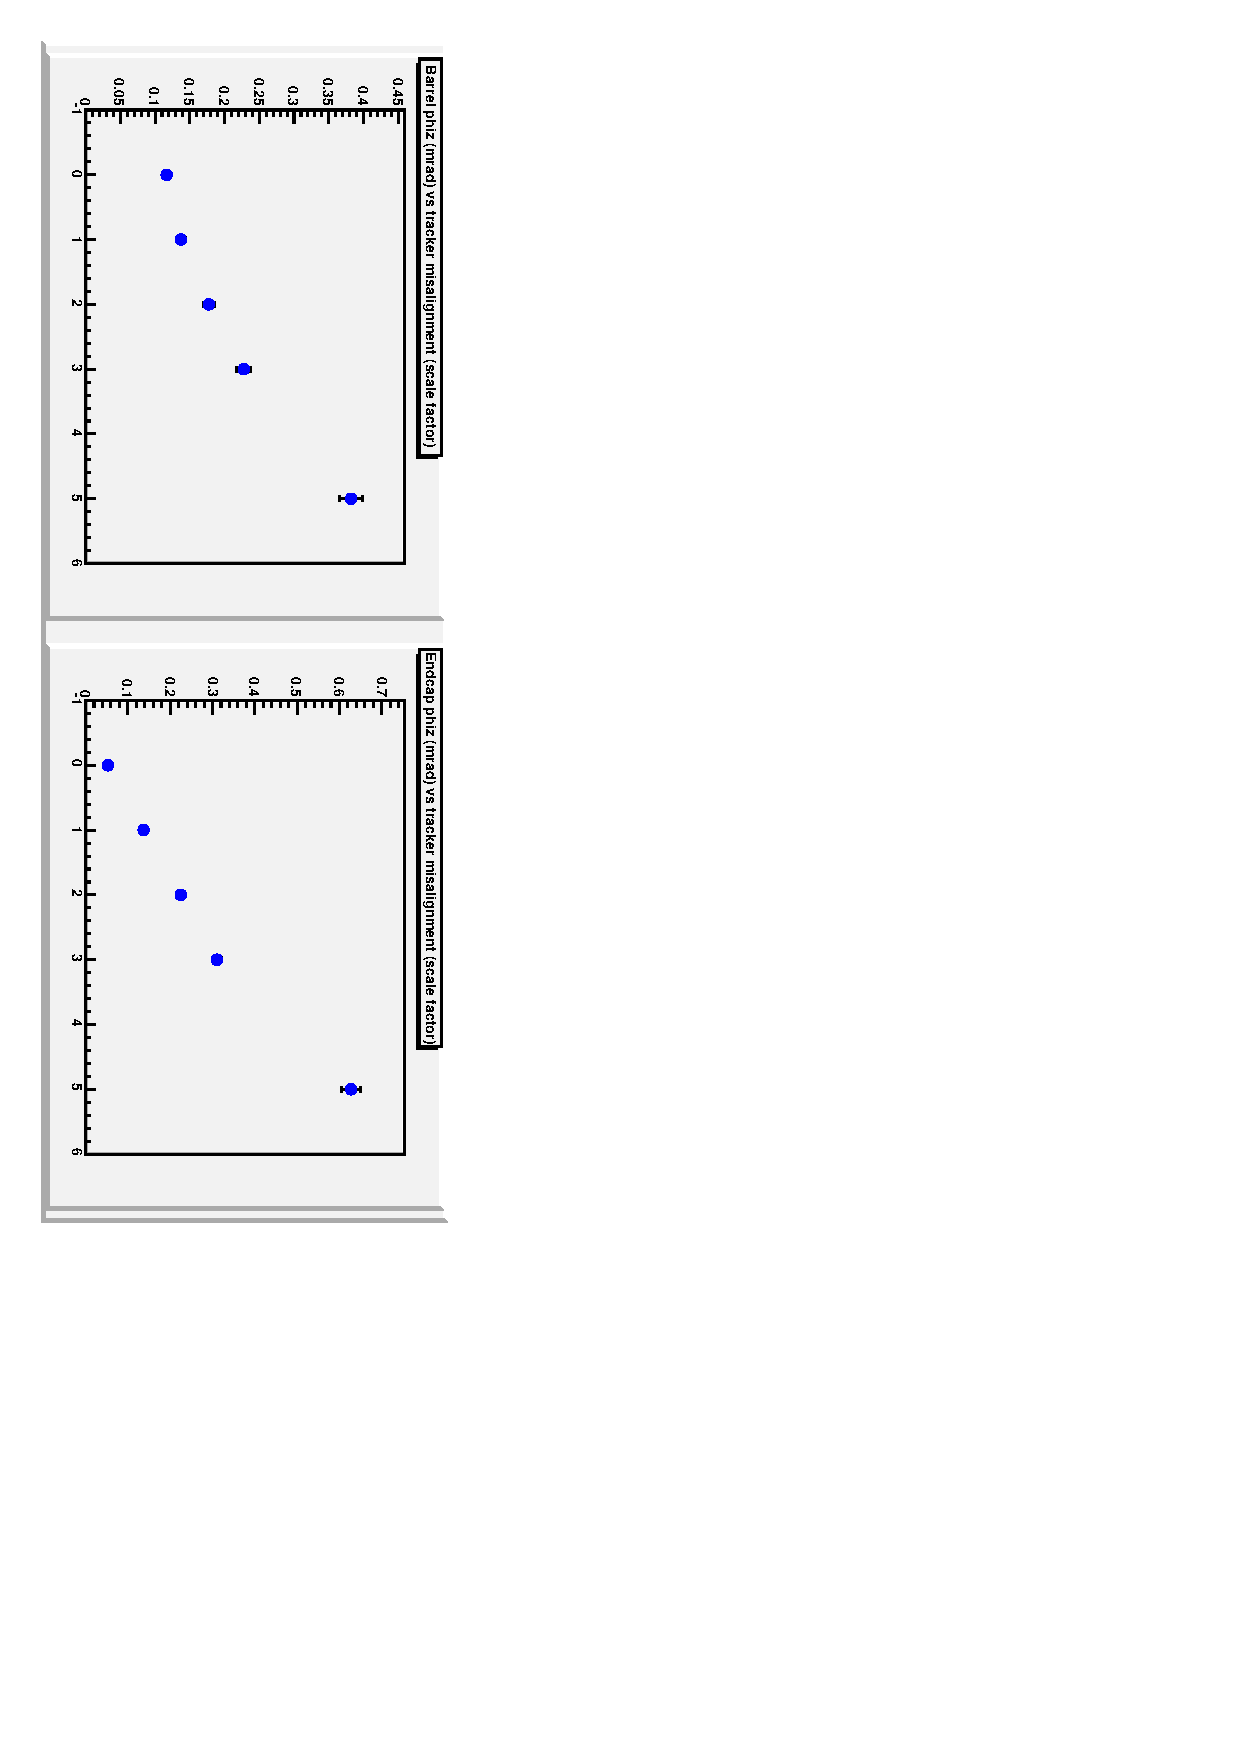
\includegraphics[height=\linewidth, angle=90]{tracker_phiz_rmsonly.pdf}
\end{columns}
\end{frame}

\begin{frame}
\frametitle{Effect of tracker misalignment (3 of 3)}
\begin{columns}
\column{0.7\linewidth}
\mbox{ } \hfill Outer endcap \hfill \hfill Inner endcap \hfill \mbox{ }

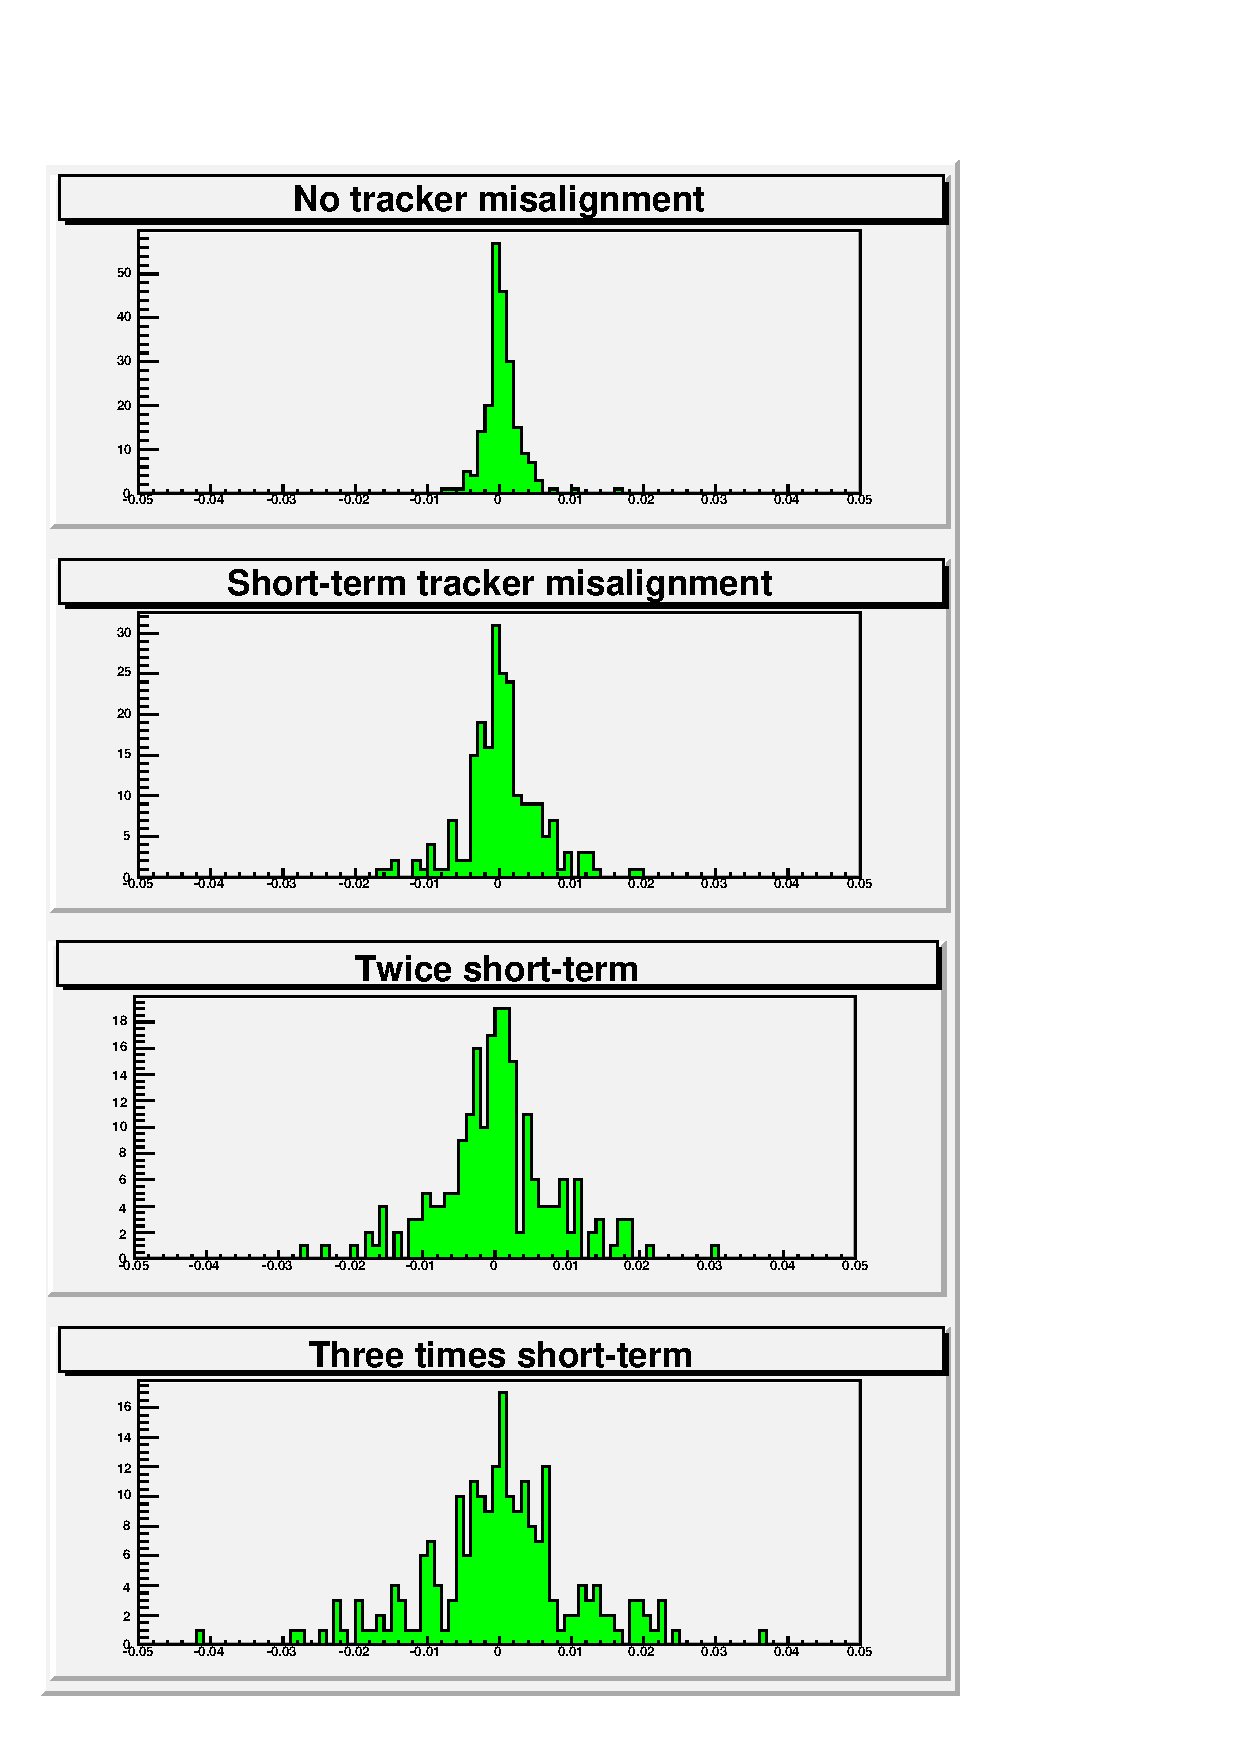
\includegraphics[width=0.5\linewidth]{trackerdep_outer_endcap.pdf}
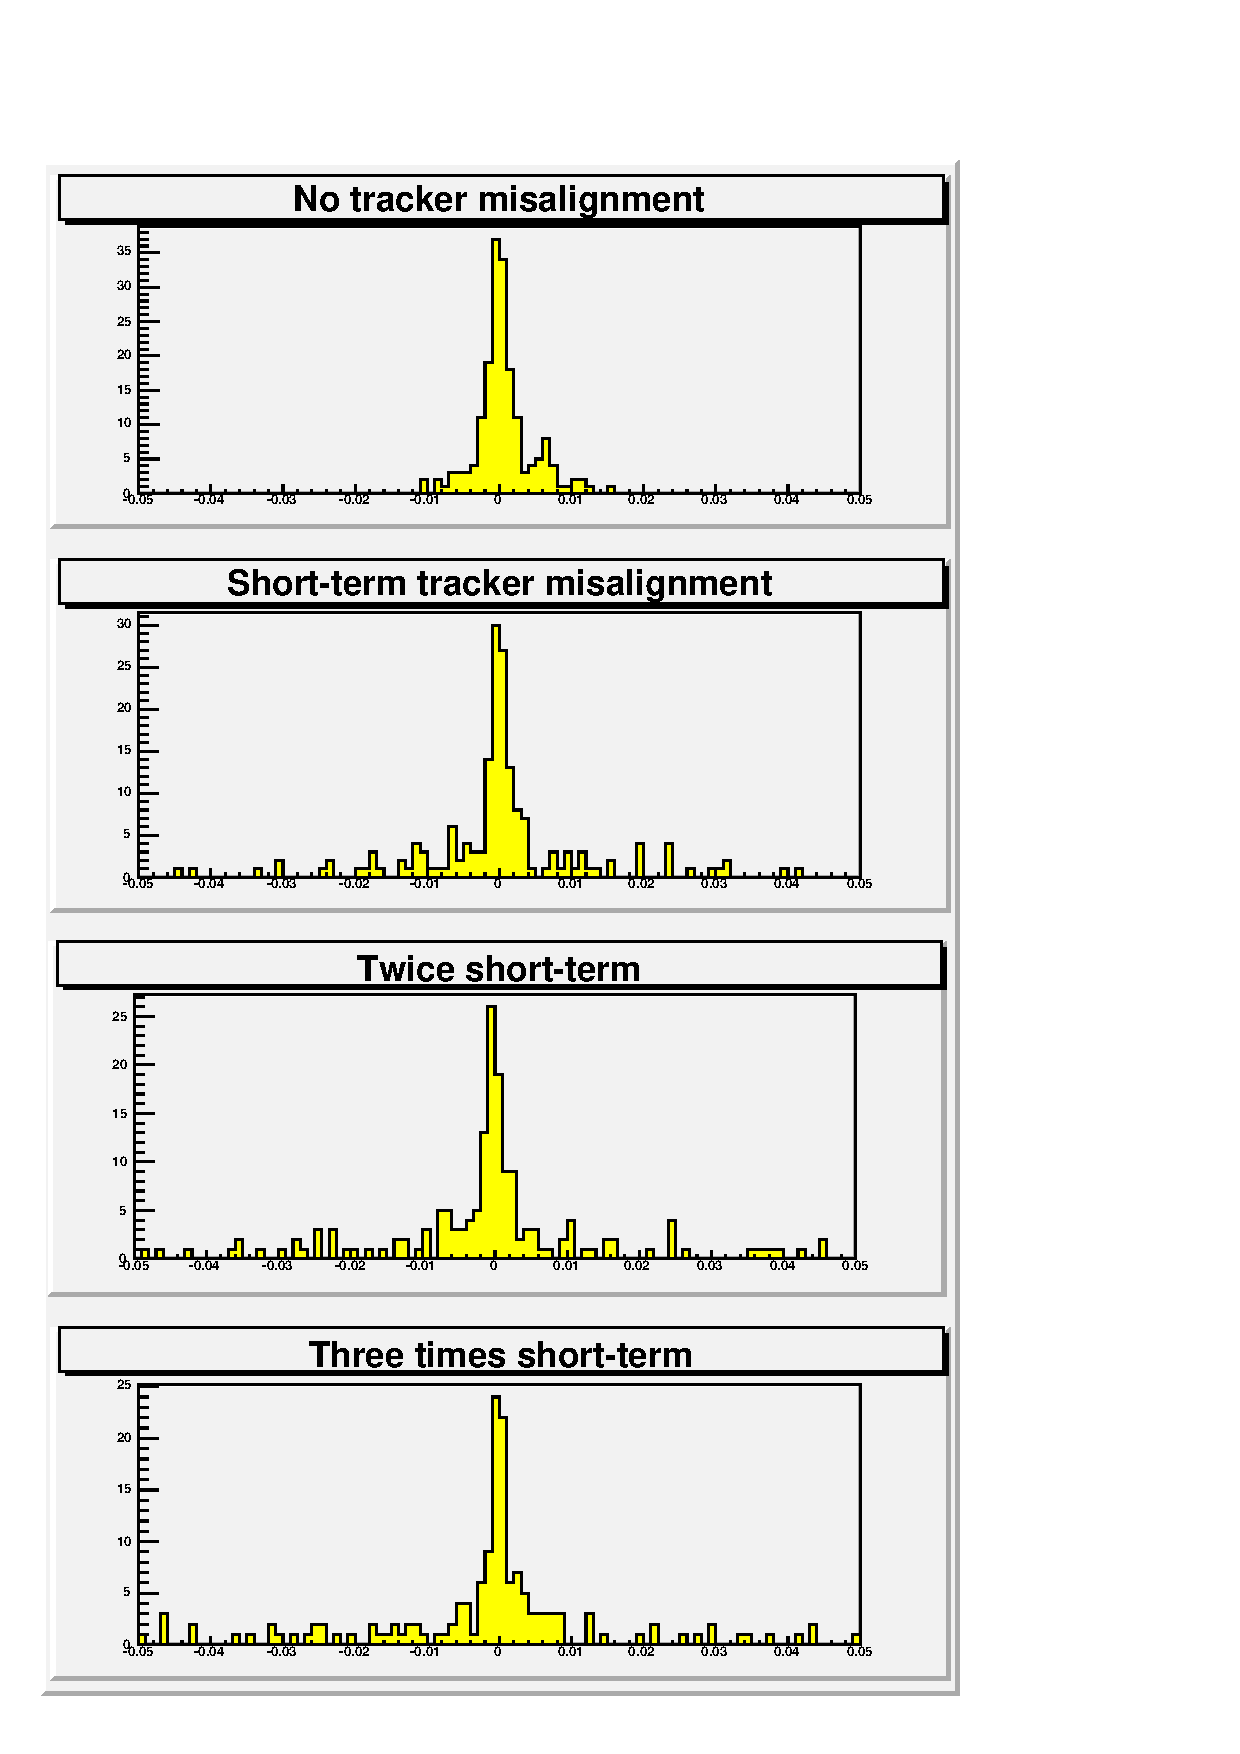
\includegraphics[width=0.5\linewidth]{trackerdep_inner_endcap.pdf}
\column{0.36\linewidth}

\mbox{\hspace{-0.5 cm}} 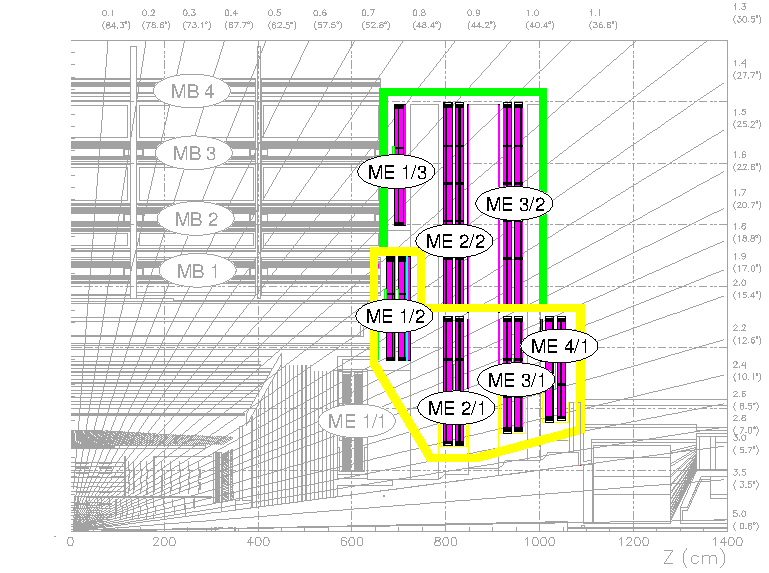
\includegraphics[width=\linewidth]{outer_inner_endcap.pdf}

\vspace{0.2 cm}
Outer endcap (1/3, 2/2, 3/2) only widens

\vspace{0.2 cm}
But inner endcap (1/2, $N$/1) gets more outliers

\vspace{0.2 cm}
May need to apply standalone procedure to these, if tracker is bad

\end{columns}
\end{frame}

\begin{frame}
\frametitle{Effect of miscalibration}
\begin{columns}
\column{0.55\linewidth}
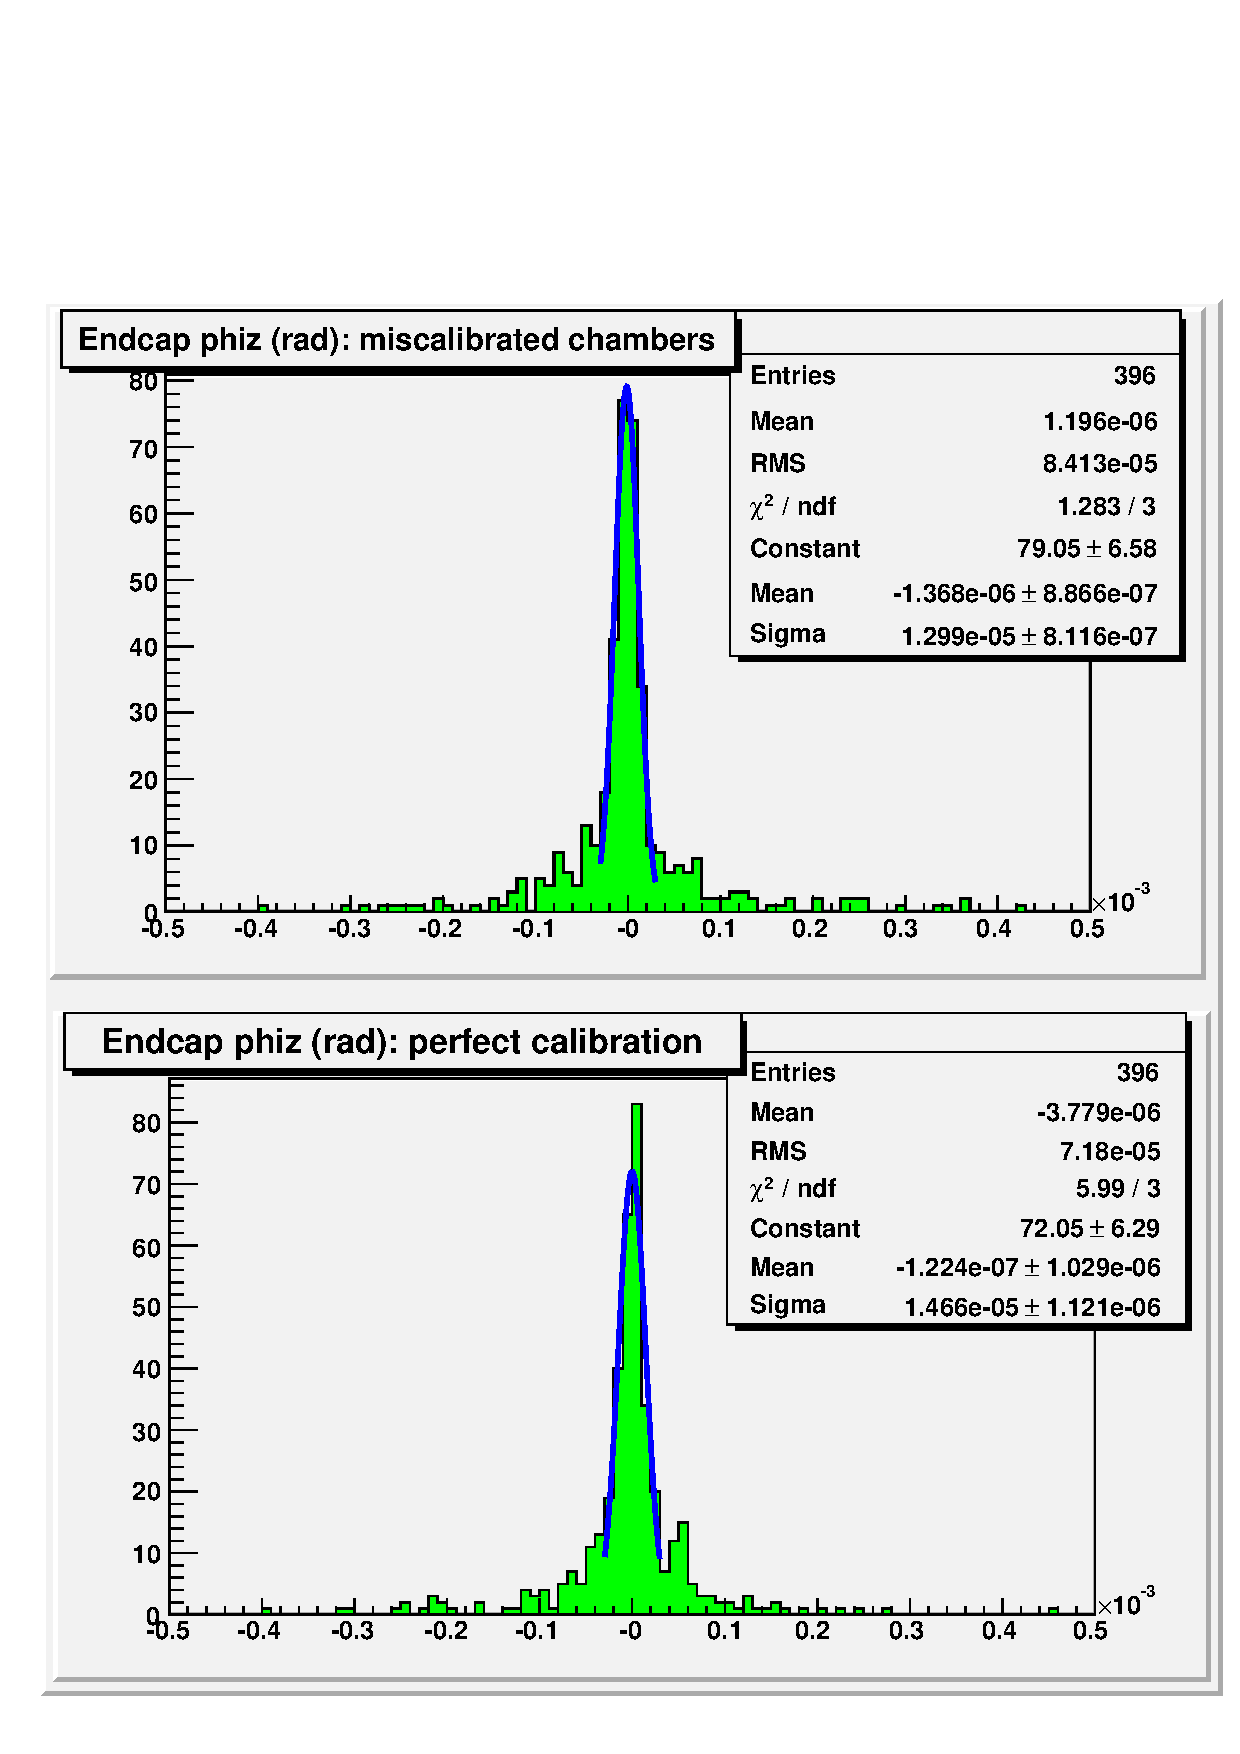
\includegraphics[width=\linewidth]{miscal_endcap_phiz.pdf}

\column{0.45\linewidth}

\vspace{-1.2 cm}
\begin{itemize}
\item 10 pb$^{-1}$ miscalibration scenario
\item Small influence on tails
\end{itemize}

\begin{center}
Barrel ($\Delta$ RMS)

\vspace{0.05 cm}
\renewcommand{\arraystretch}{1.2}
\begin{tabular}{c c | c c}
\hline\hline
$x$ & 6\% & 0\% & $\phi_x$ \\
$y$ & 1\% & 3\% & $\phi_y$ \\
$z$ & 0\% & 10\% & $\phi_z$ \\
\hline\hline
\end{tabular}

\vspace{0.5 cm}
Endcap ($\Delta$ RMS)

\vspace{0.05 cm}
\renewcommand{\arraystretch}{1.2}
\begin{tabular}{c c | c c}
\hline\hline
$x$ & 15\% & & \\
$y$ & 9\% & 3\% & $\phi_y$ \\
$z$ & 2\% & 17\% & $\phi_z$ \\
\hline\hline
\end{tabular}
\end{center}
\end{columns}
\end{frame}

\begin{frame}
\frametitle{Dependence on muon momentum}

\vspace{-1 cm}
\mbox{ } \hfill 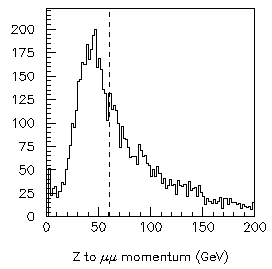
\includegraphics[width=2 cm]{p_distribution.png}

\vspace{-1.3 cm}
\begin{itemize}
\item Divide $Z\to\mu\mu$ sample along 60~GeV median
\end{itemize}

\begin{columns}
\column{0.5\linewidth}
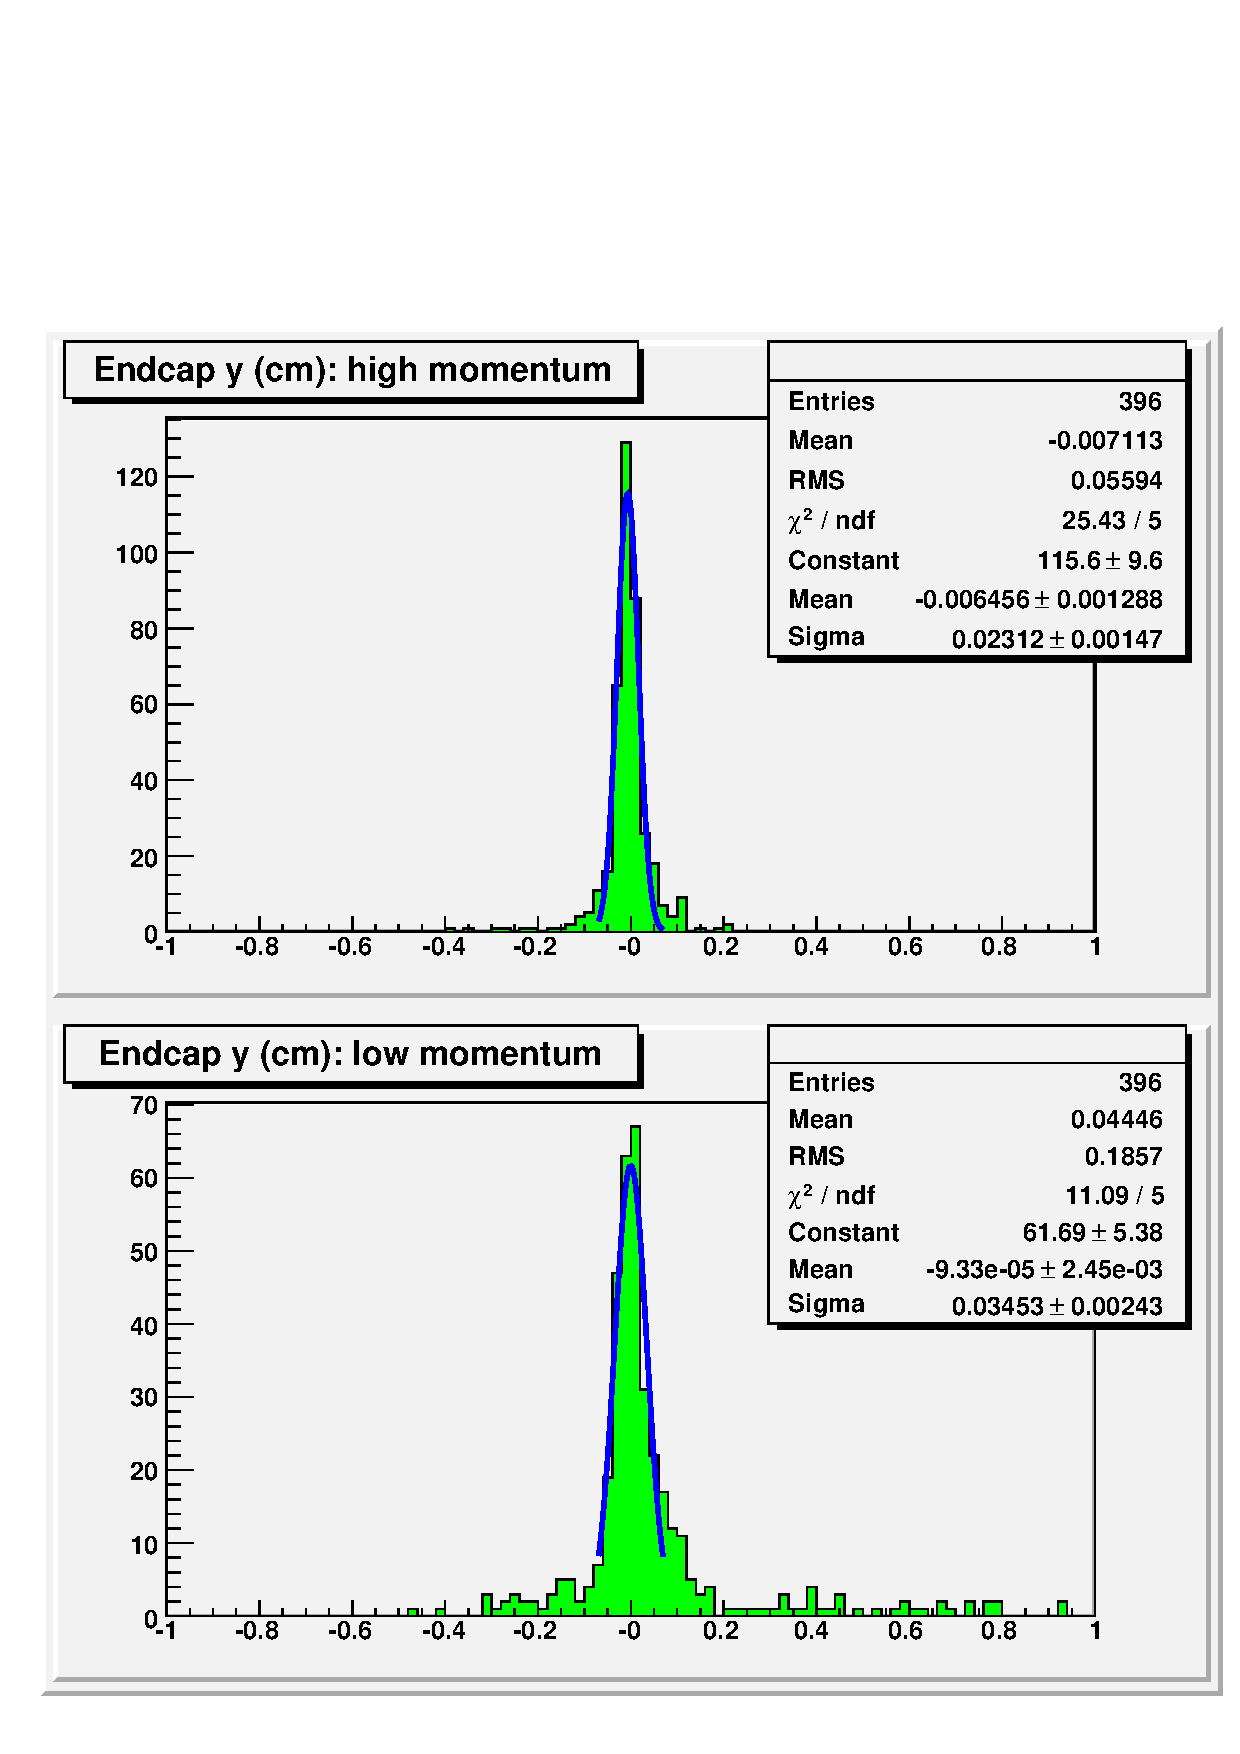
\includegraphics[width=\linewidth]{momentum_endcap_y.pdf}
\column{0.5\linewidth}
\begin{tabular}{l}
$\Delta$ Resolution \\\hline\hline
\end{tabular}

\vspace{0.3 cm}
Barrel: $<$ 5\% in each parameter

\vspace{0.2 cm}
Endcap: \begin{tabular}{c c c}
& core & RMS \\\hline
$x$ & $\times$1.5 & $\times$3 \\
$y$ & $\times$1.5 & $\times$3 \\
$z$ & $\times$3 & $\times$3 \\
$\phi_y$ & $\times$1.6 & $\times$3.5 \\
$\phi_z$ & $\times$1.2 & $\times$2
\end{tabular}

\vspace{0.2 cm}
Note asymmetric tail in $y$!

\vspace{-0.4 cm}
\begin{center}
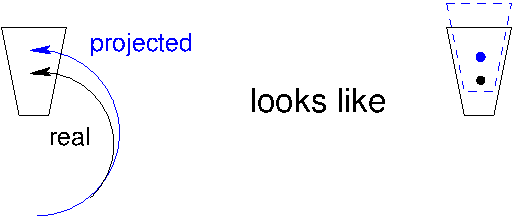
\includegraphics[width=0.8\linewidth]{momentum_y_explanation.pdf}
\end{center}
\end{columns}
\end{frame}

\section*{Beam-halo studies (Karoly)}

\begin{frame}
\begin{center}
\Huge \textcolor{blue}{Beam-halo studies (Karoly)}
\end{center}
\end{frame}

\begin{frame}
\frametitle{Alignment plans with beam-halo}
\vspace{-1.75 cm}
\mbox{ } \hfill 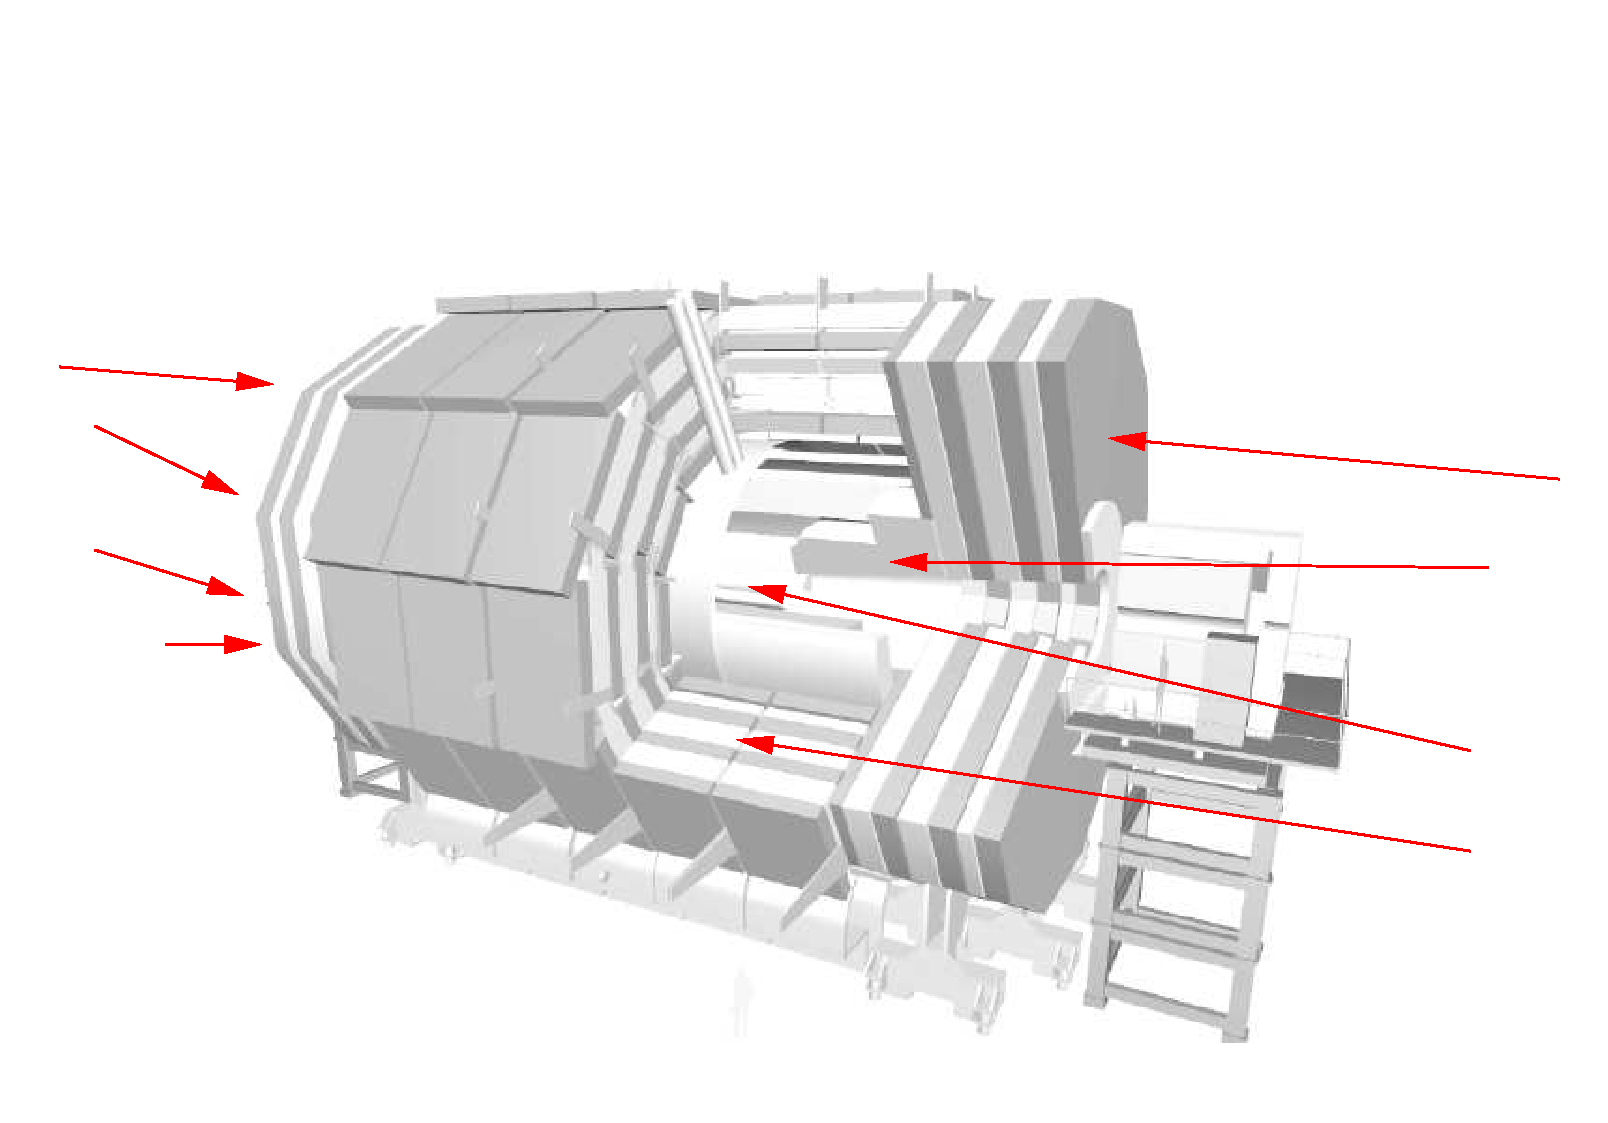
\includegraphics[width=4 cm]{beamhalo.pdf}

\vspace{-0.5 cm}
\begin{minipage}{1.05\linewidth}
\begin{itemize}\setlength{\itemsep}{0.5 cm}
\item Before first collisions

\vspace{0.1 cm}
\begin{itemize}\setlength{\itemsep}{0.3 cm}
\item Accumulate beam-halo muons from accelerator studies

with constant conditions (constant $\vec{B}(t)$, detector positions)
\item Align CSC layers; remains valid even after chambers/disks move
\item Will the rate be high enough?  To be determined\ldots
\end{itemize}

\item With collisions

\vspace{0.1 cm}
\begin{itemize}\setlength{\itemsep}{0.3 cm}
\item Combine muons from the vertex with beam-halo muons: \\ requires a new trigger (under discussion)

\item Alignment will be improved by more orthogonal tracks
\end{itemize}
\end{itemize}
\end{minipage}
\end{frame}

%% \begin{frame}
%% \frametitle{Beam-halo illumination (1 of 2)}
%% 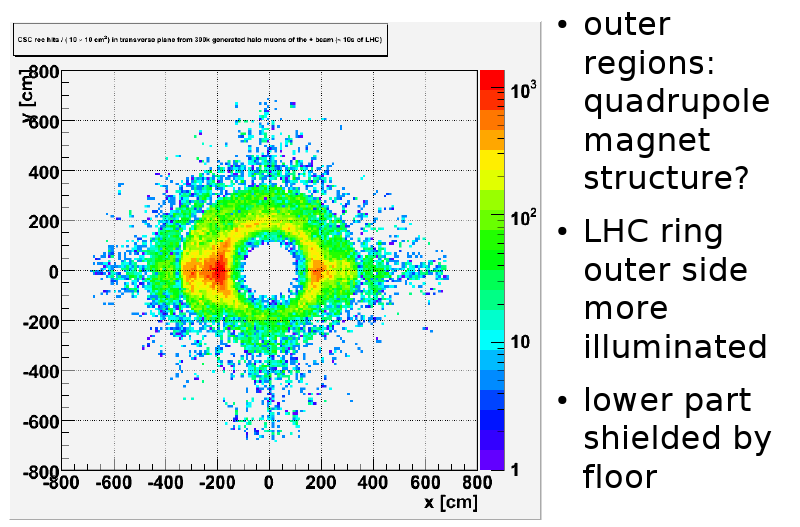
\includegraphics[width=\linewidth]{karoly_illumination.png}
%% \end{frame}

\begin{frame}
\frametitle{Beam-halo illumination}
\begin{columns}
\column{0.6\linewidth}
\vspace{0.25 cm}
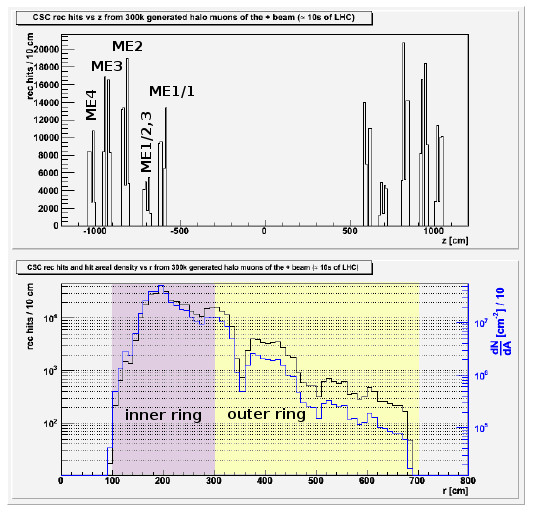
\includegraphics[width=\linewidth]{karoly_illumination2.png}
\vspace{-0.25 cm}
\begin{center}
Top: $z$ (cm) \hspace{0.5 cm} Bottom: $r$ (cm)
\end{center}

\column{0.4\linewidth}
All four stations covered

\vspace{0.2 cm}
Chambers in outer rings will get uneven statistics

\vspace{0.2 cm}
A few tracks connect both sides

\vspace{0.5 cm}
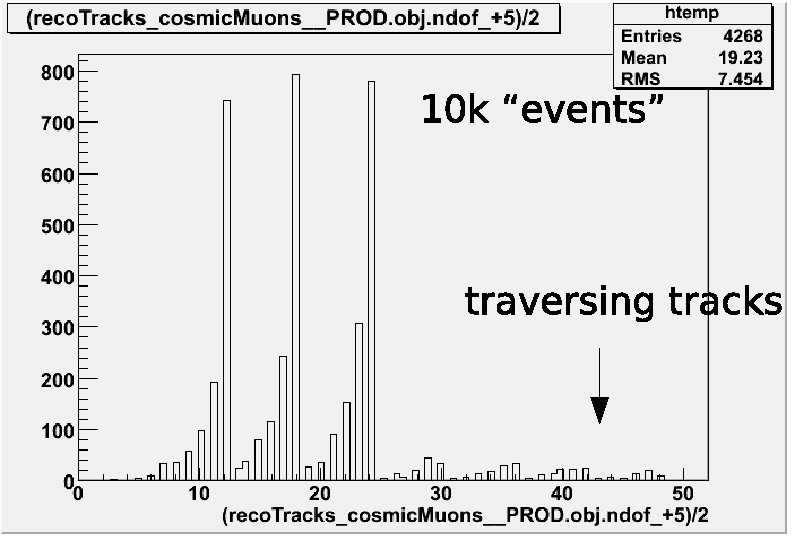
\includegraphics[width=\linewidth]{karoly_illumination3.pdf} \\
\vspace{-0.5 cm}
\begin{center}
Number of hits
\end{center}
\end{columns}
\end{frame}

%% \begin{frame}
%% \frametitle{To do}
%% \begin{center}
%% \fbox{\begin{minipage}{0.9\linewidth}
%% \begin{enumerate}\setlength{\itemsep}{0.75 cm}
%% \item Determine beam-halo rate

%% ($\to$ length of the constant-conditions time block)

%% \vspace{0.5 cm} Karoly will be presenting at the LHC Machine-Induced
%% Background Working Group to learn more from the experts
%% \end{enumerate}
%% \end{minipage}}
%% \end{center}

%% \vspace{0.5 cm}
%% \begin{itemize}\setlength{\itemsep}{0.75 cm}
%% \item Alignment simulations: can we align layers this way?

%% \item Combined beam-halo and beam-beam alignment: how much does it
%% help?
%% \end{itemize}

%% \vfill
%% \mbox{ }
%% \end{frame}

\section*{}

\begin{frame}
\frametitle{Conclusions}
\begin{itemize}\setlength{\itemsep}{0.2 cm}
\item Basic infrastructure is in place for CSA07 and beyond; we are developing monitors

\item Continuing to improve the baseline procedure

\item Problem with ME1/1, possible software bug

\item Learning quantitative relevance of systematic effects, some
of which are responsible for outliers

\vspace{0.1 cm}
\begin{itemize}\setlength{\itemsep}{0.2 cm}
\item Tracker misalignment --- important if worse than ``short-term''
\item Chamber miscalibration --- only small effects
\item Muon momentum --- degradation in endcap with 20--60~GeV
\end{itemize}

\item Karoly is making great progress with beam-halo alignment feasibility studies

\item MTCC/alignment with cosmic rays is a high priority
\end{itemize}

\label{numpages}
\end{frame}

\end{document}
